 % options:
% thesis=B bachelor's thesis
% thesis=M master's thesis
% czech thesis in Czech language
% slovak thesis in Slovak language
% english thesis in English language
% hidelinks remove colour boxes around hyperlinks

\documentclass[thesis=M,czech]{FITthesis}[2012/06/26]

\usepackage[utf8]{inputenc} % LaTeX source encoded as UTF-8

\usepackage{graphicx} %graphics files inclusion
% \usepackage{amsmath} %advanced maths
% \usepackage{amssymb} %additional math symbols

\usepackage{dirtree} %directory tree visualisation

\usepackage{nameref}
\usepackage{hyperref}
\usepackage{longtable}
\usepackage{pifont}

% % list of acronyms
% \usepackage[acronym,nonumberlist,toc,numberedsection=autolabel]{glossaries}
% \iflanguage{czech}{\renewcommand*{\acronymname}{Seznam pou{\v z}it{\' y}ch zkratek}}{}
% \makeglossaries

\newcommand{\tg}{\mathop{\mathrm{tg}}} %cesky tangens
\newcommand{\cotg}{\mathop{\mathrm{cotg}}} %cesky cotangens

\usepackage{xcolor}
\usepackage{listings}
\lstdefinelanguage{swift}
{
  morekeywords={
    func,if,then,else,for,in,while,do,switch,case,default,where,break,continue,fallthrough,return,
    typealias,struct,class,enum,protocol,var,func,let,get,set,willSet,didSet,inout,init,deinit,extension,
    subscript,prefix,operator,infix,postfix,precedence,associativity,left,right,none,convenience,dynamic,
    final,lazy,mutating,nonmutating,optional,override,required,static,unowned,safe,weak,internal,
    private,public,is,as,self,unsafe,dynamicType,true,false,nil,Type,Protocol,
  },
  morecomment=[l]{//}, % l is for line comment
  morecomment=[s]{/*}{*/}, % s is for start and end delimiter
  morestring=[b]" % defines that strings are enclosed in double quotes
}

\definecolor{keyword}{HTML}{BA2CA3}
\definecolor{string}{HTML}{D12F1B}
\definecolor{comment}{HTML}{008400}

\lstset{
  language=swift,
  basicstyle=\ttfamily,
  upquote=true,
  showstringspaces=false, % lets spaces in strings appear as real spaces
  columns=fixed,
  keepspaces=true,
  keywordstyle=\color{keyword},
  stringstyle=\color{string},
  commentstyle=\color{comment},
}




% % % % % % % % % % % % % % % % % % % % % % % % % % % % % % 
% ODTUD DAL VSE ZMENTE
% % % % % % % % % % % % % % % % % % % % % % % % % % % % % % 

\department{Katedra softwarového inženýrství}
\title{Letecké záznamy pro iOS pomocí moderních architektur a FRP}
\authorGN{Martin} %(křestní) jméno (jména) autora
\authorFN{Žid} %příjmení autora
\authorWithDegrees{Bc. Martin Žid} %jméno autora včetně současných akademických titulů
\author{Martin Žid} %jméno autora bez akademických titulů
\supervisor{Ing. Dominik Veselý}

\acknowledgements{Doplňte, máte-li komu a za co děkovat. V~opačném případě úplně odstraňte tento příkaz.}

\abstractCS{
%TOTO NENI FINALNI VERZE
Tato práce realizuje iOS aplikaci pro evidenci letů.  V první části analyzuji obdobné aplikace a předpisy pro piloty České republiky, podle nichž probíhá návrh funkcionality vytvářené aplikace. Podle návrhu je následně zvolena vhodná architektura a vytvořeno uživatelského rozhraní v podobě wireframů.

Aplikace je implementována s použitím zvolené architektury a pomocí principů FRP. V průběhu implementace aplikace jsou realizovány jednotkové testy a na konci jsou provedeny uživatelské testy. Na základě výsledků testů je aplikace upravena do finální podoby.

V poslední části práce popisuji výhody a nevýhody, které přinesly postupy FRP. Také hodnotím časovou a implementační náročnost oproti standardním postupům a architektuře MVC. 

V~práci jsem vytvořil funkční iOS aplikaci s využitím moderní architektury a principů FRP. Aplikace bude sloužit pilotům České republiky pro elektronickou evidenci letů a bude jim také ulehčovat administrativu s evidencí spojenou.

V~příloze této diplomové práce je možné nalézt všechny zdrojové kódy jak aplikace, tak i testů společně s~vytvořenými wireframy.
}

\abstractEN{Sem doplňte ekvivalent abstraktu Vaší práce v~angličtině.}

\placeForDeclarationOfAuthenticity{V~Praze}
\declarationOfAuthenticityOption{4} %volba Prohlášení (číslo 1-6)
\keywordsCS{mobilní aplikace pro evidenci letů, iOS, Swift, FRP, ReactiveCocoa, MVVM architektura}
\keywordsEN{flight records mobile application, iOS, Swift, FRP, ReactiveCocoa, MVVM architecture}

\begin{document}

% \newacronym{CVUT}{{\v C}VUT}{{\v C}esk{\' e} vysok{\' e} u{\v c}en{\' i} technick{\' e} v Praze}
% \newacronym{FIT}{FIT}{Fakulta informa{\v c}n{\' i}ch technologi{\' i}}

\begin{introduction}
V dnešní době, kdy existují mobilní aplikace na téměř vše, mě zarazil fakt, že u pilotů tomu tak nemusí být. Aplikace na evidenci letů samozřejmě existují, však je tu hned několik problémů. Tyto aplikace jsou často velice drahé, nemusí odpovídat leteckým přepisům České republiky nebo nemají vyhovující funkcionalitu.

Z tohoto důvodu jsem se rozhodl vytvořit iOS aplikaci na evidenci letů. Tato aplikace bude pomáhat pilotům zaznamenávat elektronicky své lety, bude také kontrolovat předpisy a umožňovat export do formátu pro tisk.

Začínám analýzou podobných aplikací, a to pro zařízení iOS i Android. Poté navrhuji vhodnou funkcionalitu a vytvářím návrh uživatelského rozhraní.

Dalším tématem, které ve své práci řeším, jsou softwarové architektury při vývoji iOS aplikace. Zde analyzuji alternativy k architektuře MVC ve spojení s funkcionálně reaktivním programováním neboli FRP.

Tuto analýzu následně aplikuji v praxi, kdy se zvolenou architekturou a FRP implementuji společně s jednotkovými testy dříve zmíněnou aplikaci. Nakonec aplikaci podrobím uživatelským testům a podle jejich výsledků
upravím aplikaci do finální podoby.

V poslední části své práce se snažím zhodnotit postupy FRP společně se mnou zvolenou moderní architekturou a jejich časovou a implementační náročnost oproti klasickému MVC.
\end{introduction}

\chapter{Cíl práce}
Cílem této práce je navrhnout a implementovat aplikaci k evidenci letů pro platformu iOS, a to pomocí postupů FRP (funkcionálně reaktivního programování) a s využitím moderní softwarové architektury jako např. MVVM nebo VIPER.  Tato aplikace bude sloužit pilotům České republiky k elektronické evidenci letů. Tento cíl je rozdělen do několika podúkolů.

V první části analyzuji podobné aplikace pro evidenci letů, a to jak pro platformu iOS, tak i pro Android. Na základě této analýzy navrhnu vhodnou funkcionalitu pro vytvářenou aplikaci. Podle navržených funkcionalit si zvolím architekturu  a navrhnu uživatelské rozhraní v podobě wireframů.

V dalším kroku aplikaci implementuji pomocí postupů FRP a se zvolenou architekturou. V průběhu realizace aplikace budou vytvářeny také testy a dokumentace aplikace.

Dále bude aplikace podrobena uživatelským testům, podle kterých bude vhodně upravena.

V poslední části budu popisovat výhody a nevýhody, které přinesly postupy FRP. Budu také hodnotit časovou a implementační náročnost oproti standardním postupům a architektuře MVC. 


\chapter{Tvorba iOS aplikací}

\section{Možnosti vývoje}
Vývoj iOS aplikace je možný hned několika způsoby, každý má své výhody a nevýhody, právě ty bych rád v této kapitole rozebral. Mezi možné způsoby vývoje bych rád zmínil nativní aplikace, hybridní aplikace a mobilní webové aplikace.

\subsection{Nativní aplikace}
Nativní aplikace jsou vyvíjeny specificky pro jednu platformu. Díky tomu mají přístup ke všem funkcím daného zařízení jako např. GPS, kamera nebo kontakty. Mohou fungovat i pouze offline, tedy bez nutnosti internetového připojení. \cite{Nielsen}

Však pokud bychom chtěli aplikaci distribuovat na více platforem, tak s tímto přístupem by bylo nutné vytvořit pro každou platformu vlastní aplikaci. To by prodloužilo vývoj a znesnadnilo následnou údržbu aplikací.

Co se týče iOS vývoje, je možné si zvolit z dvou programovacích jazyků -- Objective-C nebo Swift. \cite{objc} \cite{swift}

\subsection{Hybridní aplikace}
Hybridní aplikace jsou aplikace tvořené nejčastěji pomocí HTML5 a JavaScriptu, následně jsou spuštěné v nativním kontejneru. \cite{saleforce} Jako příklad je možné uvést např. Apache Cordova. Tento kontejner umožňuje přístup k funkcím daného přístroje, podporuje použití aplikace offline a dává možnost publikace vytvořené aplikace do obchodu tzv. app store. \cite{cordova}

Však výhodou nativních aplikacím proti hybridním je to, že jsou vytvářeny přesně pro danou platformu, a tudíž jejich vzhled a výkon bude vždy lepší. \cite{upwork}

\subsection{Mobilní webové aplikace}
Poslední možností jsou mobilní webové aplikace. Tyto aplikace jsou pouze upravené webové stránky do podoby a chování nativních aplikací. Přestože běží pouze v prohlížeči, mohou mít i tyto aplikace přístup k určitým (ne však ke všem) nativním funkcím. \cite{Nielsen}

Tím, že jsou mobilní webové aplikace spouštěny v prohlížeči a nejsou stahovány přes obchody, je ulehčena údržba a vývoj, protože si uživatel nemusí vždy stahovat novou verzi aplikace.

Však tento postup má i své nevýhody. Jak již bylo zmíněno dříve, aplikace nemá přístup ke všem nativním funkcím daného přístroje. S dalším problémem se můžeme setkat u offline ukládání dat, a to se zabezpečením, které nemusí být tak dokonalé nebo uživatelsky přívětivé, jako u nativních aplikací.  \cite{saleforce}

\subsection{Zvolené řešení}
Pro svou práci jsem si zvolil možnost nativní mobilní aplikace z důvodu zaměření pouze na platformu iOS. Bude se tedy jednat pouze o jednu aplikaci, která bude moci využít všech nativních funkcionalit, výkonu i vzhledu.

\section{Architektury při tvorbě iOS aplikací}
Při tvorbě iOS aplikace je možné si vybrat z několika architektur. V této kapitole budu rozebírat pouze MVC, MVVM a VIPER.

\subsection{MVC}
Architektura MVC je zkratka pro \uv{Model-View-Controller} neboli tři komponenty, ze kterých se architektura skládá. Jedná se o softwarovou architekturu, které se velice často používá při tvorbě aplikací s uživatelským rozhraním. \cite{MVCMozilla}
\begin{itemize}
\item $Model$ definuje jaká data aplikace obsahuje, a pokud dojde k jakékoliv změně, tak informuje buď $Controller$ nebo $View$ (tzv. své observery). \cite{MVCGoogle}
\item $View$ vrstva je prezentována samotnému uživateli. Tedy jsou zde zobrazena aplikační data a je zachycována uživatelova práce s aplikací.\cite{MVCMozilla}
\item $Controller$ je vrstva mezi $View$ a $Model$ zajišťující logiku aplikace. Stará se o prezentaci změn do $View$ pokud se změní $Model$. Zároveň provádí úpravy v $Modelu$ při uživatelově manipulaci s $View$.  \cite{MVCGoogle}
\end{itemize}

Však co se týče iOS vývoje, vrstvy $View$ a $Controller$ jsou téměř spojeny, protože $Controller$ je příliš úzce zapojený do životního cyklu $View$, což následně způsobuje velký nárůst $Controlleru$.\cite{Orlov}

Základní myšlenku MVC a MVC při vývoji iOS aplikace ukazují obrázky \ref{fig:mvc} (převzato a přeloženo z originálu \cite{mvc-pic}) a \ref{fig:mvc-apple} (převzato a přeloženo z originálu \cite{mvc-apple-pic}).

MVC je základní architekturou pro tvorbu iOS aplikací. Není však jedinou možností.

\begin{figure}[h]\centering
 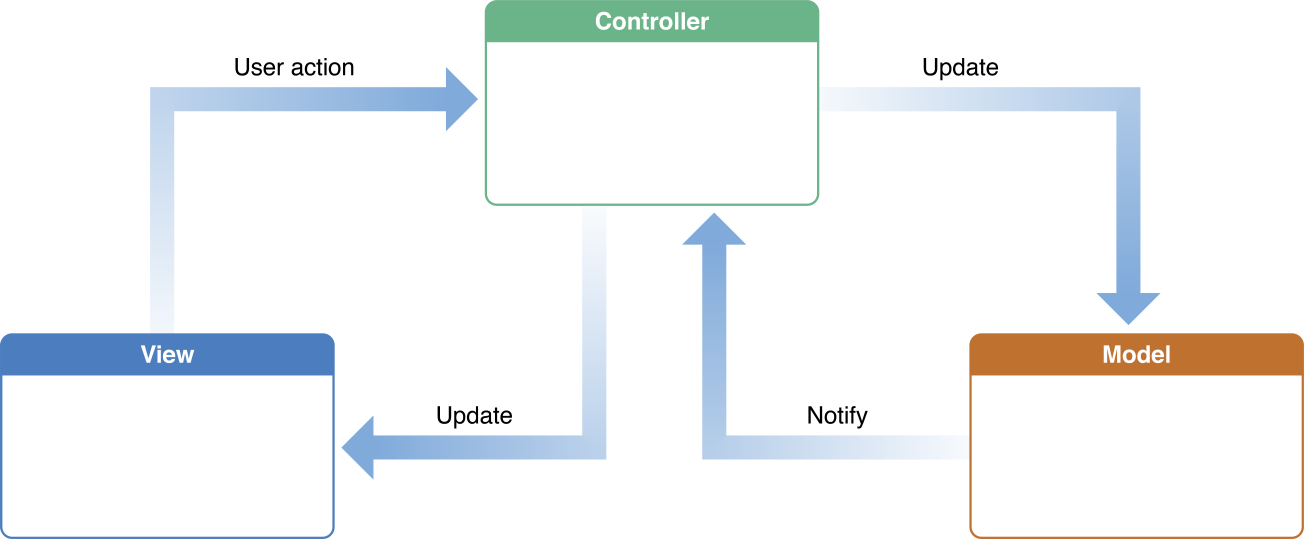
\includegraphics[width=0.99\textwidth]{./pictures/architektury/model_view_controller}
 \caption[Model-View-Controller diagram]{Model-View-Controller diagram}\label{fig:mvc}
\end{figure}

\begin{figure}[h]\centering
 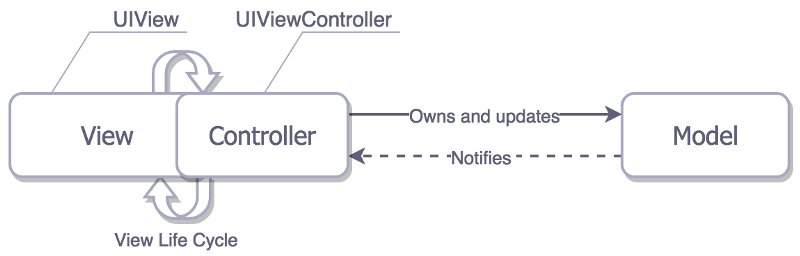
\includegraphics[width=0.99\textwidth]{./pictures/architektury/appleMVC}
 \caption[Model-View-Controller při vývoji iOS aplikace]{Model-View-Controller při vývoji iOS aplikace}\label{fig:mvc-apple}
\end{figure}

\subsection{MVVM}
Architektura MVVM má obdobné koncepce jako MVC. Jedná se také o zkratku, tentokrát \uv{Model-View-ViewModel}. \cite{MVVMMicrosoft}
\begin{itemize}
\item $Model$ je totožný s $Model$ vrstvou architektury MVC, jedná se tedy o datovou část aplikace.
\item $View$ prezentuje aplikační data uživateli a monitoruje jeho akce. Však, jak již bylo zmíněno dříve, u iOS aplikací se jedná spíše o vrstvu\\ $View/Controller$. Tato vrstva obsahuje pouze minimum logiky aplikace a reaguje hlavně na $ViewModel$.  \cite{Morrison}
\item $ViewModel$ spojuje $View$ a $Model$ a zajišťuje hlavní logiku aplikace. $ViewModel$ tedy komunikuje s $Modelem$ a jeho metodami a následně připravuje data pro $View$. Obsahuje také implementaci funkcí, které reagují a zpracovávají akce uživatele např. kliknutí na tlačítko. \cite{MVVMMicrosoft}
\end{itemize}

Tedy pro shrnutí rozdílů MVC a MVVM u iOS bych zmínil to, že iOS MVC má ve výsledku téměř jen dvě vrstvy $View/Controller$ a $Model$. Když potom uvažujeme architekturu MVVM, $View/Controller$  je opravdu pouze jednou vrstvou a mezi ní a $Modelem$ je vložena nová vrstva $ViewModel$, která je spojuje, a do které je přesunuta i většina aplikační logiky.

Mezi výhody architektury MVVM oproti MVC patří např.:
\begin{itemize}
\item poskytnutí návrhového principu tzv. separation of concerns, neboli oddělení zájmů;
\item zlepšení možnosti testovatelnosti aplikace.
\end{itemize}

Architekturu MVVM zobrazuje obrázek \ref{fig:mvvm} (převzato a přeloženo z originálu \cite{mvvm-pic}).

\begin{figure}[h]\centering
 \includegraphics[width=0.99\textwidth]{./pictures/architektury/MVVM}
 \caption[Model-View-ViewModel architektura]{Model-View-ViewModel architektura}\label{fig:mvvm}
\end{figure}

\subsection{VIPER}
VIPER je poslední analyzovanou možností, co se týče architektur. I zde je název složen z prvních písmen jednotlivých vrstev architektury, tedy \uv{View, Interactor, Presenter, Entity, Router}.
\begin{itemize}
\item $View$  zobrazuje data uživateli a předává uživatelovi vstupy vrstvě $Presenter$.
\item $Interactor$ obsahuje logiku aplikace spojenou s daty ($Entity$).
\item $Presenter$ vrstva má na starosti $View$ logiku. Reaguje tedy na uživatelovy akce a komunikuje s vrstvou $Interactor$, od ní také přijímá nová data. \cite{Orlov}
\item $Entity$ jsou datové objekty aplikace přístupné pouze části $Interactor$.
\item $Router$ obsahuje navigační logiku. \cite{VIPER}
\end{itemize}

Mezi výhody architektury VIPER znovu patří např.:
\begin{itemize}
\item dobré rozdělení odpovědností;
\item zlepšení možnosti testovatelnosti aplikace. \cite{Orlov}
\end{itemize}

Tato architektura však může být zbytečně složitá pro menší aplikace. \cite{Orlov}

Architekturu VIPER zobrazuje obrázek \ref{fig:viper} (převzato a přeloženo z originálu \cite{viper-pic}).

\begin{figure}[h]\centering
 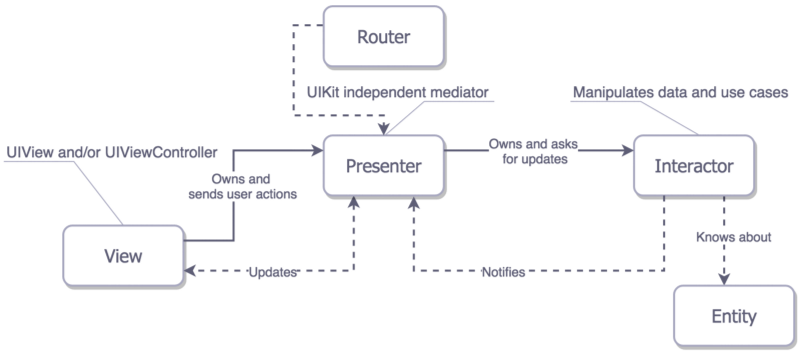
\includegraphics[width=0.99\textwidth]{./pictures/architektury/viper.png}
 \caption[VIPER architektura]{VIPER architektura}\label{fig:viper}
\end{figure}

\section{Tvorba uživatelského rozhraní}
Při vývoji iOS aplikace existují tři možnosti, jak vytvořit uživatelské rozhraní -- $storyboard$, $Xib$ a kód. Každá z těchto možností má své výhody a nevýhody. \cite{iOSUI}

\subsection{Storyboard}

\begin{figure}[]\centering
 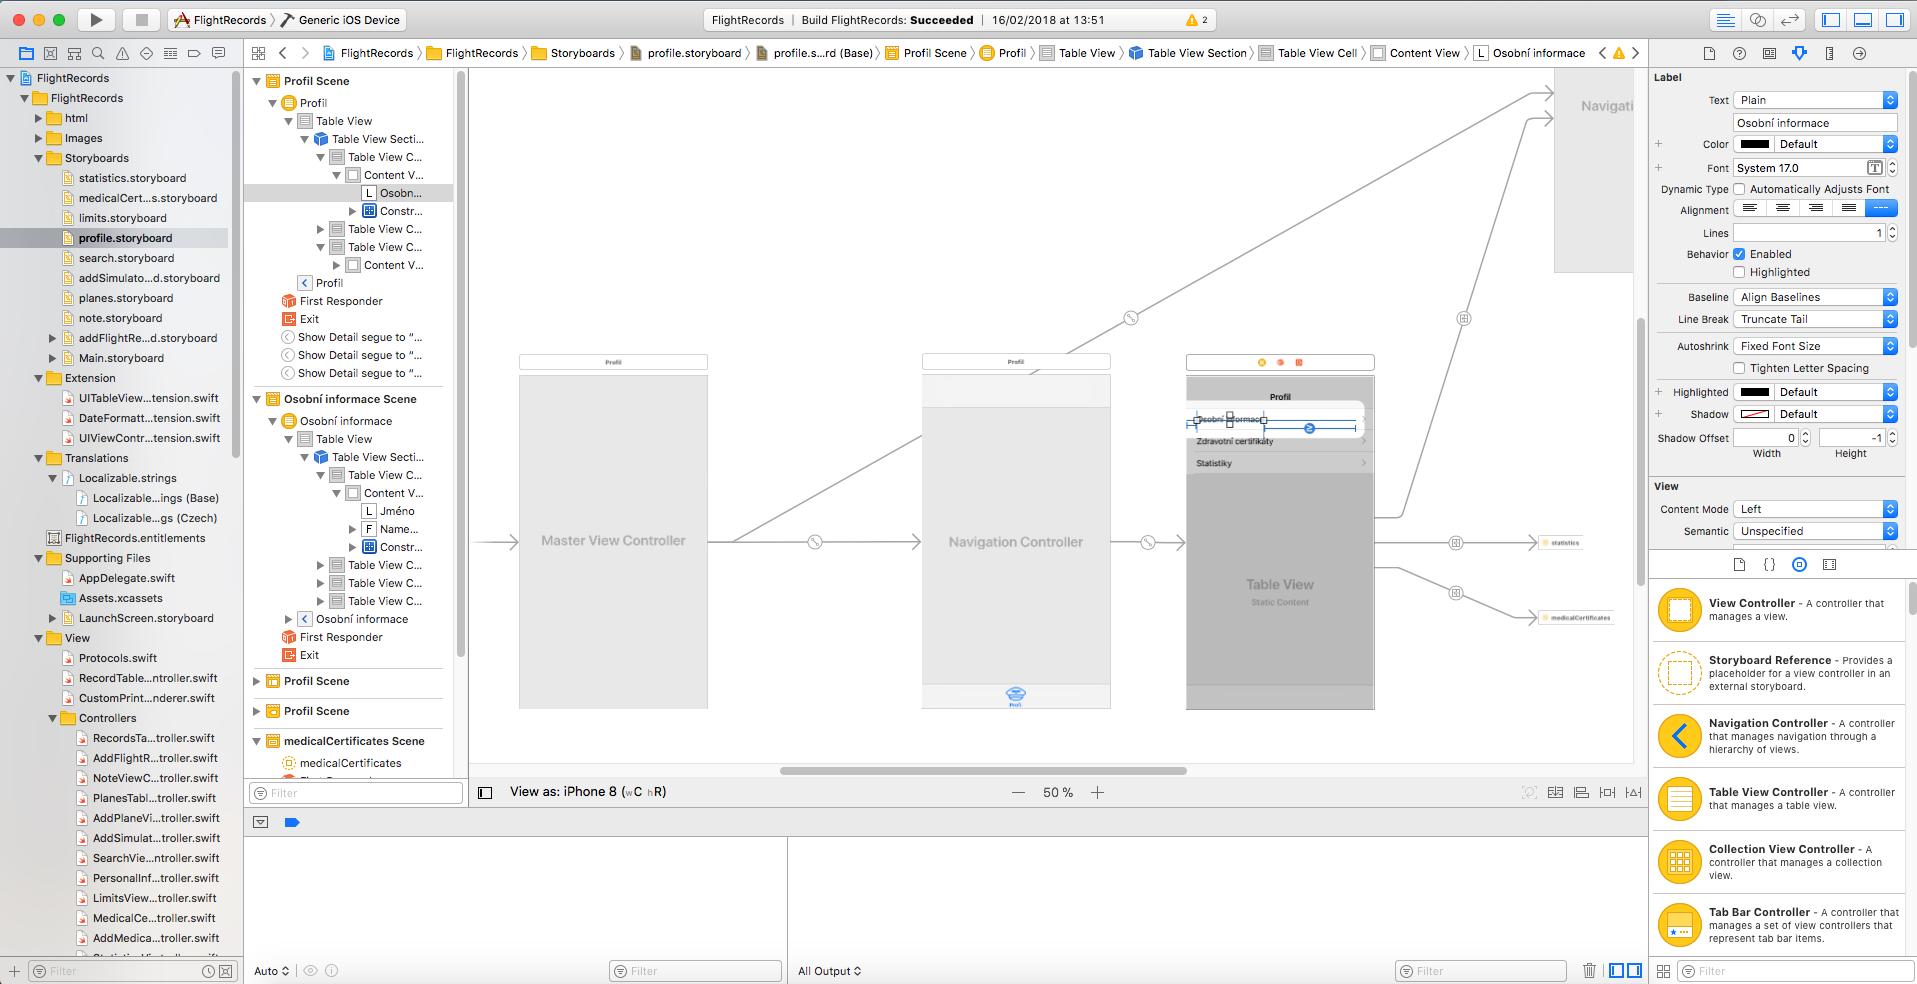
\includegraphics[width=0.99\textwidth]{./pictures/storyboard}
 \caption[Storyboard]{Storyboard (pouze ilustrační)}\label{fig:SB}
\end{figure}

$Storyboard$ představuje grafickou reprezentaci uživatelského rozhraní -- zobrazuje jednotlivé obrazovky, jejich obsah a propojení těchto obrazovek. Xcode mají zabudovaný editor pro tvorbu a úpravu $storyboardu$ (viz. obrázek \ref{fig:SB}). Jednotlivé prvky jsou vkládány jednoduchým přetažením a je u nich možné upravit obsah, velikost, barvu a podobně, ihned v editoru. Tento editor také umožňuje propojení jednotlivých prvků a jejich akcí s kódem aplikace. \cite{SB}

Mezi výhody $storyboarů$ patří rychlost tvorby uživatelské rozhraní, což zahrnuje i rychlou tvorbu prototypů aplikace. Dále vizuální zobrazení, nejen prvků, ale také propojení jednotlivých obrazovek, a to bez nutnosti kompilování aplikace. 

Nevýhodou $storyboardů$ může být výkon při více nebo složitějších obrazovkách. Tento problém se však dá zredukovat rozdělením obrazovek do více $storyboard$ souborů. Další nevýhodou je problematické znovupoužití jednotlivých prvků (obrazovek) nebo komplikovaná práce v týmu způsobená složitým spojením změn při verzování (i tento problém řeší z části více souborů se $storyboardy$). Posledním nedostatkem je to, že ne vše se dá vytvořit ve $storyboardu$ (hlavně dynamické prvky) a z toho důvodu dochází k tomu, že část uživatelského rozhraní je v kódu a část ve $storyboardu$. \cite{iOSUI} \cite{dominik}

\subsection{Xib}
$Xib$ je starším přístupem pro tvorbu uživatelského rozhraní iOS aplikací než $storyboardy$, starší však neznamená zastaralý. Vytváří se jednoduché $view$ elementy stejným způsobem jako o $storyboardů$. Právě tato skutečnost přináší stejné výhody i problémy, s tím rozdílem, že se jedná o drobnější prvky, což ulehčuje např. verzování, znovupoužitelnost nebo nezpůsobuje zpomalovaní vývojového prostředí Xcode. \cite{iOSUI} \cite{dominik}

\subsection{Uživatelské rozhraní v kódu}
Poslední možností jak tvořit uživatelské rozhraní je vlastní kód. Tento způsob přináší mnoho výhod (hlavně tím, že redukuje nedostatky $storyboardů$ a $Xib$), ale má i své nevýhody.

Mezi výhody vlastního kód patří: znovupoužitelnost, bezproblémová práce ve více lidech (verzování) a to, že se vše nachází na jedno místě. 

Nevýhodou vytváření uživatelské rozhraní v kódu je rychlost tvorby bez možnosti svižného vytvoření prototypu aplikace. Dále také tento přístup postrádá vizuálnost a vyžaduje kompilaci. \cite{iOSUI} \cite{dominik}

\subsection{Zvolené řešení}
Pro tvorbu aplikace vytvářené v rámci této diplomové práce, jsem si zvolil možnost tvorby uživatelského rozhraní pomocí $storyboardů$. Tato volba vyplývá z výše zmíněných výhod $storyboardů$ a z toho důvodu, že aplikaci budu vytvářet sám.

\section{Funkcionálně reaktivní programování}
Funkcionálně reaktivní programování je kombinací funkcionálního a reaktivního programování, díky němuž dokáže aplikace dynamicky měnit stav a chování v závislosti na událostech přicházejících za daný čas. \cite{nayebi2016swift}

Pro vysvětlení, co je to reaktivní programování, cituji André Staltze: \uv{reaktivní programování je programování s asynchronními datovými toky}. \cite{Ztaltz2014}

Na spojení funkcionální a reaktivního programování může dívat i jako na návrhový vzor $observer$. \cite{Blackheath2016} Pozorujeme tedy např. určité vstupní pole, tlačítko nebo i dotaz na server a jsme informování o každé změně v podobě asynchronního datového toku. Na tyto datové toky je možné aplikovat funkcionální programování. Je tedy možné toky:
\begin{itemize}
\item spojovat ($merge$),
\item filtrovat ($filter$) např. pouze události, které nás zajímají,
\item mapovat ($map$) jeden tok na nový, a další. \cite{Ztaltz2014}
\end{itemize}

\subsection{FRP frameworky pro iOS}
V této kapitole jsou pouze rozebrány základy jednotlivých frameworků, podrobnější vysvětlení (zvoleného frameworku) společně s ukázkami je k nalezení v kapitole \nameref{chap:realizace}.

\subsubsection{ReactiveSwift}
ReactiveSwift je prvním frameworkem pro iOS podporující FRP. Obsahuje řadu základních prvků ($Signal$, $SignalProducer$, $Property$, $Action$\ldots) a operátorů podporujících myšlenku \uv{streams of values over time}. \cite{ReactiveSwift}

\subsubsection{ReactiveCocoa}
ReactiveCocoa je další z FRP frameworků pro iOS. ReactiveCocoa rozšiřuje různé aspekty Apple Cocoa frameworku základními prvky frameworku ReactiveSwift. Umožňuje vazbu na prvky uživatelského rozhraní, u interaktivních prvků napojuje $Signal$ a $Action$ pro kontrolu událostí a změn. Dále také umožňuje vytvářet signály na volání metod (např. i pro UIKit třídy). \cite{ReactiveCocoa}

\subsubsection{RxSwift}
RxSwift je Swift verzí knihovny Reactive Extensions (Rx). \cite{RxSwift} Tato knihovna umožňuje vytvářet aplikace založené na událostech a asynchronních datových tocích pomocí tzv. Observables. \cite{RxNET} I přesto, že RxSwift není striktně FRP frameworkem, \cite{ReactiveExtensionsDocs} je zde uváděn, a to z důvodu velkého využití knihovny Reactive Extensions i na jiných platformách např.: JavaScript, C\#, Python. \cite{ReactiveExtensions}

\section{Perzistence dat}
Perzistence dat, neboli jejich uchování a uložení, je velice důležitou funkcionalitou většiny aplikací. V této kapitole jsou rozebírány tři možnosti zajišťující perzistenci dat iOS aplikací -- Core Data, iCloud a Realm.

\subsection{Core Data}
Core Data je Apple framework, který má na starosti model vrstvu aplikace. Stará se o životní cyklus objektů, jejich vztahy (objektový graf) i perzistenci. \cite{coredata}

Core Data má více možností jakým způsobem data uložit např. SQLite a XML. Jedná se tedy o uložení dat na disku daného zařízení.  \cite{CoreDataPersistentTypes}

Výhodou tohoto frameworku je to, že je zcela zdarma a má podporu přímo v Xcode. \cite{CoreDataXcode}

\subsection{iCloud}
iCloud je cloudové úložiště od společnosti Apple. Umožňuje ukládat aplikační data i dokumenty a přistupovat k nim na všech Apple zařízeních a na webu. \cite{iCloud}

Při vývoji iOS aplikací se pro využití iCloudu používá framework CloudKit. CloudKit zajišťuje rozhraní pro komunikaci dané aplikace a iCloudu. \cite{CloudKitDoc} Poskytuje ověření uživatele, tři druhy databáze -- soukromou, veřejnou a sdílenou. Dále také analytický nástroj CloudKit Dashboard, který umožňuje analýzu dat, měření aktivity uživatelů a další. \cite{CloudKit}

CloudKit je dostupný pro členy Apple Developer programu. \cite{AppleDeveloperProgram} Tento program stojí ročně v přepočtu 2150 Kč. \cite{AppleDeveloperProgramPrice} 

\subsection{Realm}
Realm, s oficiální stránkou \url{https://realm.io}, je multiplatformní mobilní databáze, která je připravená pro jazyky Java (Android), Swift, Objective-C, JavaScript a Xamarin. Hlavní myšlenkou je kontejner objektů tzv. Realm. V těchto kontejnerech jsou uložena data, na které je možné se dotazovat, tyto data filtrovat a podobně. Na rozdíl od klasických např. SQL databází, zde pracujeme přímo s \uv{živými} objekty, tedy pokud máme instanci Realm objektu a cokoliv v aplikaci tuto instanci změní, tato změna je ihned viditelná.

Realm je rozdělený na dvě části -- mobilní databáze Realm (Realm Mobile Database) a objektový server Realm (Realm Object Server). Jak je již z názvů možné usuzovat mobilní databáze je pouze na mobilním zařízení, jedná se tedy o offline uložení dat. Pokud však chceme data např. sdílet na více zařízení, je možné se připojit na objektový server Realm a s tím se synchronizovat. Realm se řídí strategii \uv{nejprve offine} -- čtení a zápis probíhá nejprve lokálně a až poté probíhá synchronizace se serverem.

Jedna aplikace může využívat hned několik Realm kontejnerů, a to jak lokální, tak i vzdálené, kde každý z nich může mít různá oprávnění pro různé uživatele.

Realm Mobile Database je open source, tedy zdarma. \cite{realmOverview}

\chapter{Analýza evidence letů}
\section{EASA}
EASA, neboli European Aviation Safety Agency, je agentura spadající pod Evropskou Unii, která má na starosti technické přepisy, bezpečnost, regulace a certifikace v oboru letectví. \cite{EU} 

Pro tuto diplomovou práci je EASA důležitá, protože vydává i pokyny např. pro evidenci letů nebo limity odlétaných hodin. \cite{EASARegulations}

\subsection{Pokyny pro evidenci letů}
Pokyny pro evidenci letů udává předpis FCL.050. Tento předpis specifikuje povinné položky každého leteckého záznamu. \cite{FCL} 

\uv{
Každý záznam letů by měl obsahovat minimálně tyto informace:
\begin{enumerate}
\item osobní informace: jméno a adresu pilota;
\item každý záznam letu by měl obsahovat:
	\begin{itemize}
	\item jméno velícího pilota (PIC -- Pilot-in-command),
	\item datum letu,
	\item čas a místo odletu a příletu,
	\item typ, značku, model, variantu a registraci letadla,
	\item označení zda je letadlo jednomotorové (SE -- single engine) nebo vícemotorové (ME -- multi engine),
	\item čas letu,
	\item celkový čas letu;
	\end{itemize}
\item každý záznam z výcvikového zařízení pro simulaci letu (FSTD -- flight simulation training devices) by měl obsahovat:
	\begin{itemize}
	\item typ a kvalifikační číslo výcvikového zařízení,
	\item instrukce výcvikového zařízení pro simulaci letu,
	\item datum,
	\item čas,
	\item celkový čas;
	\end{itemize}
\item funkce pilota:
	\begin{itemize}
	\item velící pilot (včetně sólového, studenta (Student PIC) nebo velícího pilota pod dohledem (PICUS -- pilot-in-command under supervision)),
	\item druhý pilot,
	\item dvojí pilot (dual),
	\item instruktor (FI -- Flight Instructor) nebo zkoušející (FE -- Flight Examiner);
	\end{itemize}
\item provozní podmínky -- pokud se let uskutečnil v noci nebo pokud byl prováděn podle pravidel pro let podle přístrojů.
\end{enumerate}
} \cite{FCL} (překlad vlastní)

\subsection{Limity}
Limity letového času a času ve službě obsahuje předpis ORO.FTL.210.

\uv{Celková doba služby, na kterou může být člen posádky přidělen, nesmí překročit:
\begin{enumerate}
\item 60 hodin služby za 7 po sobě jdoucích dnů;
\item 110 hodin služby za 14 po sobě jdoucích dnů; a 
\item 190 hodin služby za 28 po sobě jdoucích dnů, rozdělených co nejrovnoměrněji během tohoto období.
\end{enumerate}
Celkový čas, na který je jedinec přidělen jako člen provozní posádky, nesmí překročit:
\begin{enumerate}
\item 100 hodin letu za 28 po sobě jdoucích dnů;
\item 900 hodin letu v kalendářním roce; a
\item 1000 hodin letu během 12 po sobě jdoucích kalendářních měsících.
\end{enumerate}
Poletová služba se počítá do doby služby.
} \cite{FTL} (překlad vlastní)

\subsection{Zdravotní certifikáty}
Informace o zdravotních certifikátech obsahuje předpis Part-MED. Certifikáty jsou tří druhů -- zdravotní certifikát třídy 1 (Class 1 medical certificate), zdravotní certifikát třídy 2 (Class 2 medical certificate) a zdravotní certifikát pro licence na lehká letadla (LAPL -- Light Aircraft Pilot Licence). Každý z těchto certifikátů má jinak nastavenou dobu platnosti a je pro jiné typy pilotních licencí.

LAPL certifikát je pouze pro pilotní licence na lehká letadla. Platnost je 60 měsíců u pilotů do věku 40 let, poté je platnost pouze 24 měsíců.

Zdravotní certifikát třídy 2 je pro pilotní licence PPL (Private Pilot Licence), SPL (Sailplane Pilot Licence) a BPL (Balloon Pilot Licence), tedy pro piloty soukromých letadel, kluzáků a balónů. Platnost licence se znovu odvíjí od věku pilota -- 60 měsíců u pilotů do věku 40 let, následně 24 měsíců do věku 50 let a nakonec platnost licence klesá na 12 měsíců.

Zdravotní certifikát třídy 1 je certifikát nejvyšší úrovně. Je pro pilotní licence CPL (Commercial Pilot Licence), MPL (Multi-crew Pilot Licence) a ATPL (Airline Transport Pilot Licence), tedy pro piloty komerčních, vícečlenných a dopravních letadel. Platnost licence je 12 měsíců. To neplatí u pilotů starších 40 let, létajících jednopilotní komerční lety s cestujícími nebo u pilotů starších 60 let, zde se platnost licence snižuje na 6 měsíců. \cite{CAA}

\section{Analýza existujících aplikací pro evidenci letů}
Tato kapitola se zabývá analýzou již existujících aplikací pro evidenci letů. Pro analýzu bylo vybráno pět aplikací -- tři pro iOS a dvě pro platformu Android.
\begin{enumerate}
\item LogTen Pro X -- iOS aplikace v angličtině vyvíjená společností Coradine Aviation. \cite{appStoreLogTen}
\item Logbook Pro Aviation Flight Log for Pilots -- druhá iOS aplikace, také v angličtině, vytvořená NC Software, Inc. \cite{appStoreLogbookPro}
\item Safelog Pilot Logbook -- poslední z analyzovaných iOS aplikací. I tato aplikace je v anglickém jazyce. Publikována Dauntless Software. \cite{appStoreSafeLog}
\item FlyLogio - Pilot Logbook -- česká aplikace vyvinutá pro platformu Android společností FlyLogio.com. \cite{googleFlyLogio}
\item Smart Logbook -- anglická Andriod aplikace vydána firmou Kviation, Inc. \cite{googleSmartLogbook}
\end{enumerate}

\begin{figure}[]\centering
 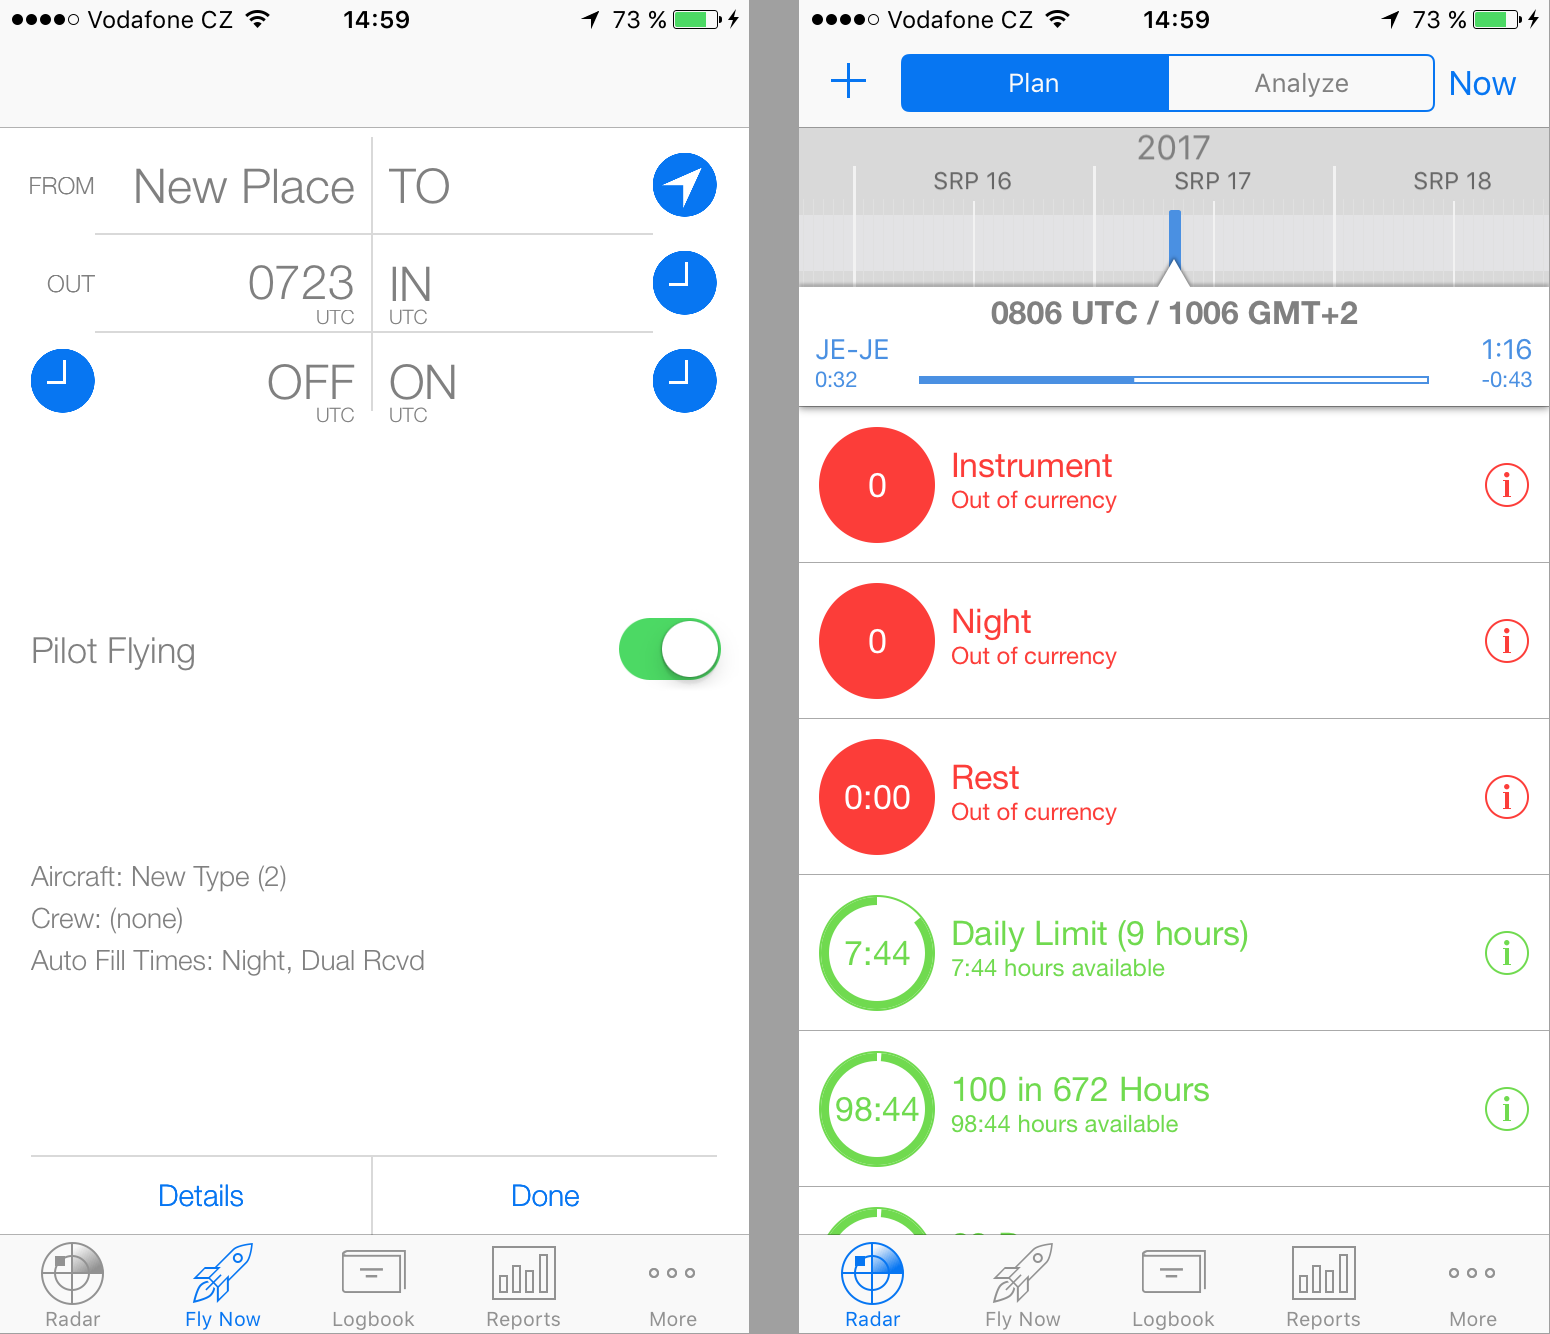
\includegraphics[width=0.99\textwidth]{./pictures/existujiciAplikace/LogTenProX}
 \caption[LogTen Pro X]{LogTen Pro X}\label{fig:LogTenProX}
\end{figure}

\begin{figure}[]\centering
 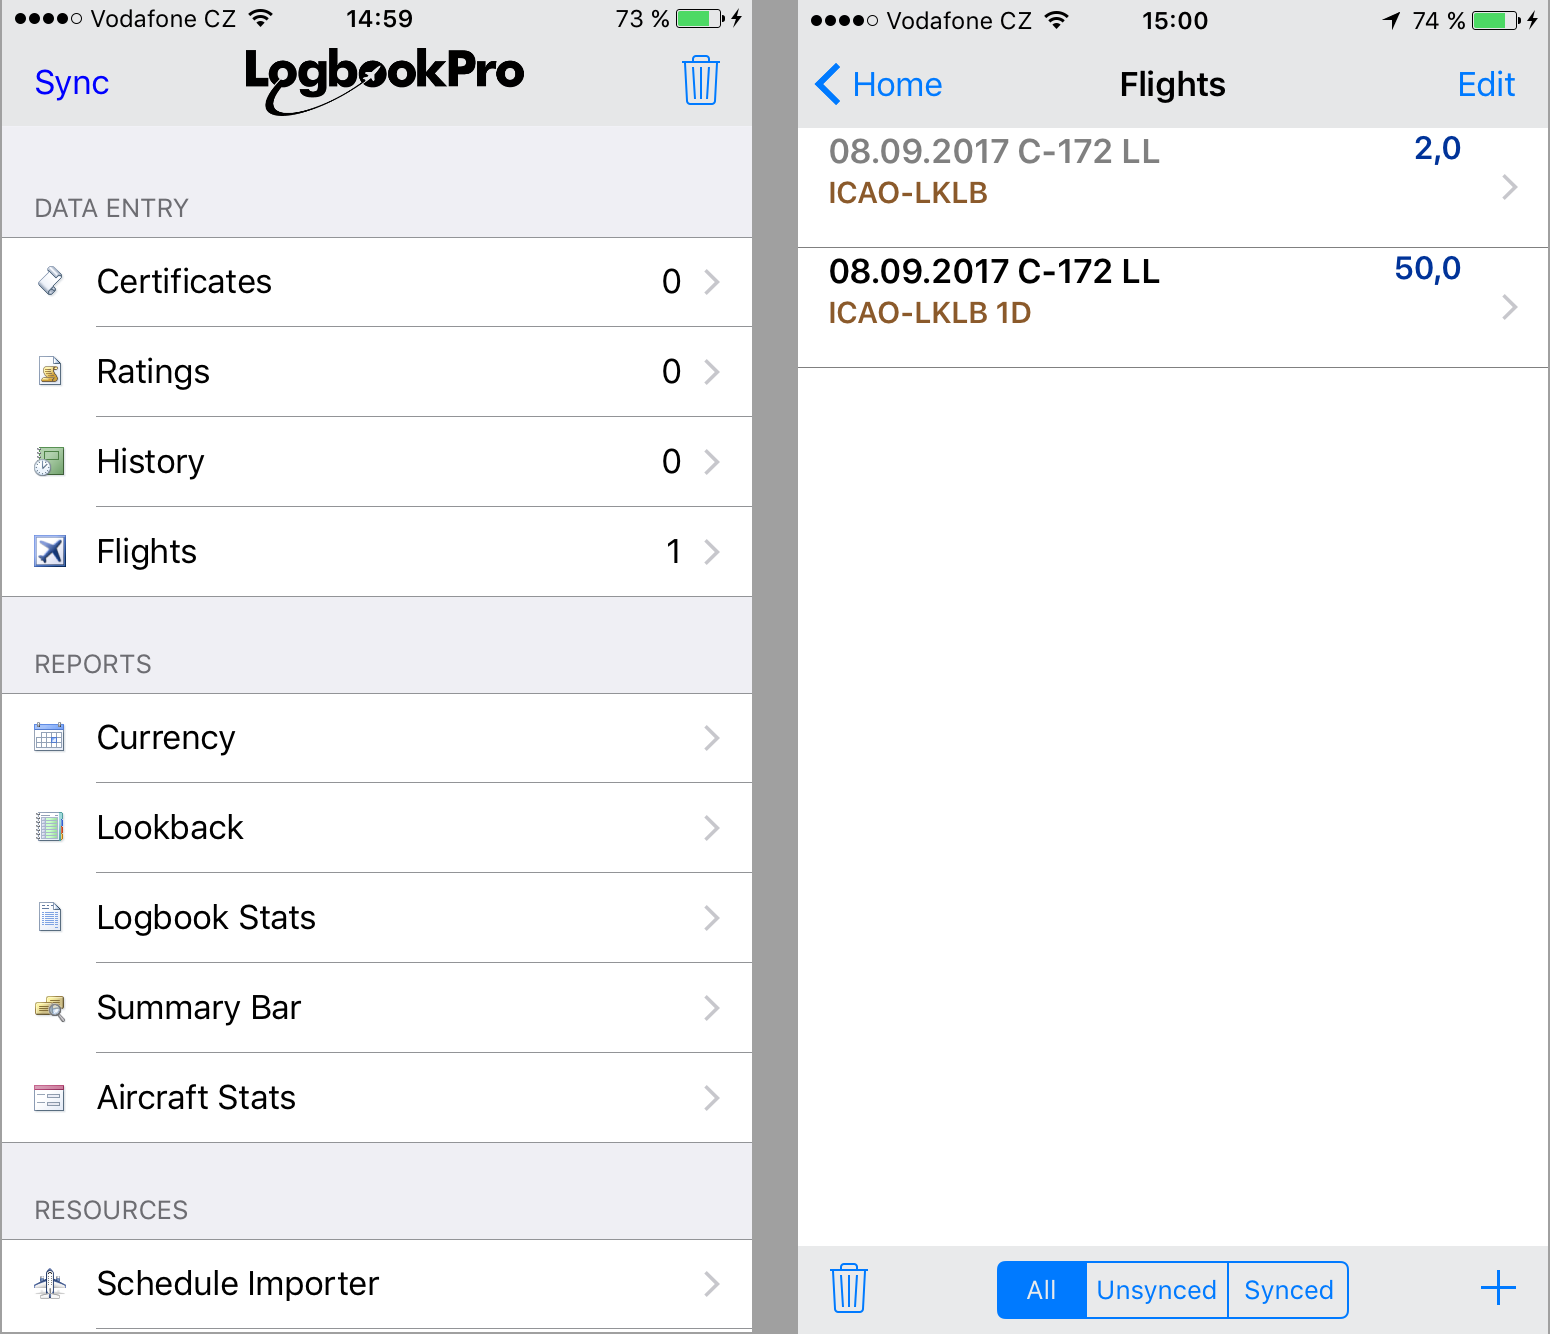
\includegraphics[width=0.99\textwidth]{./pictures/existujiciAplikace/LogbookPro}
 \caption[Logbook Pro Aviation Flight Log for Pilots]{Logbook Pro Aviation Flight Log for Pilots}\label{fig:LogbookPro}
\end{figure}

\begin{figure}[]\centering
 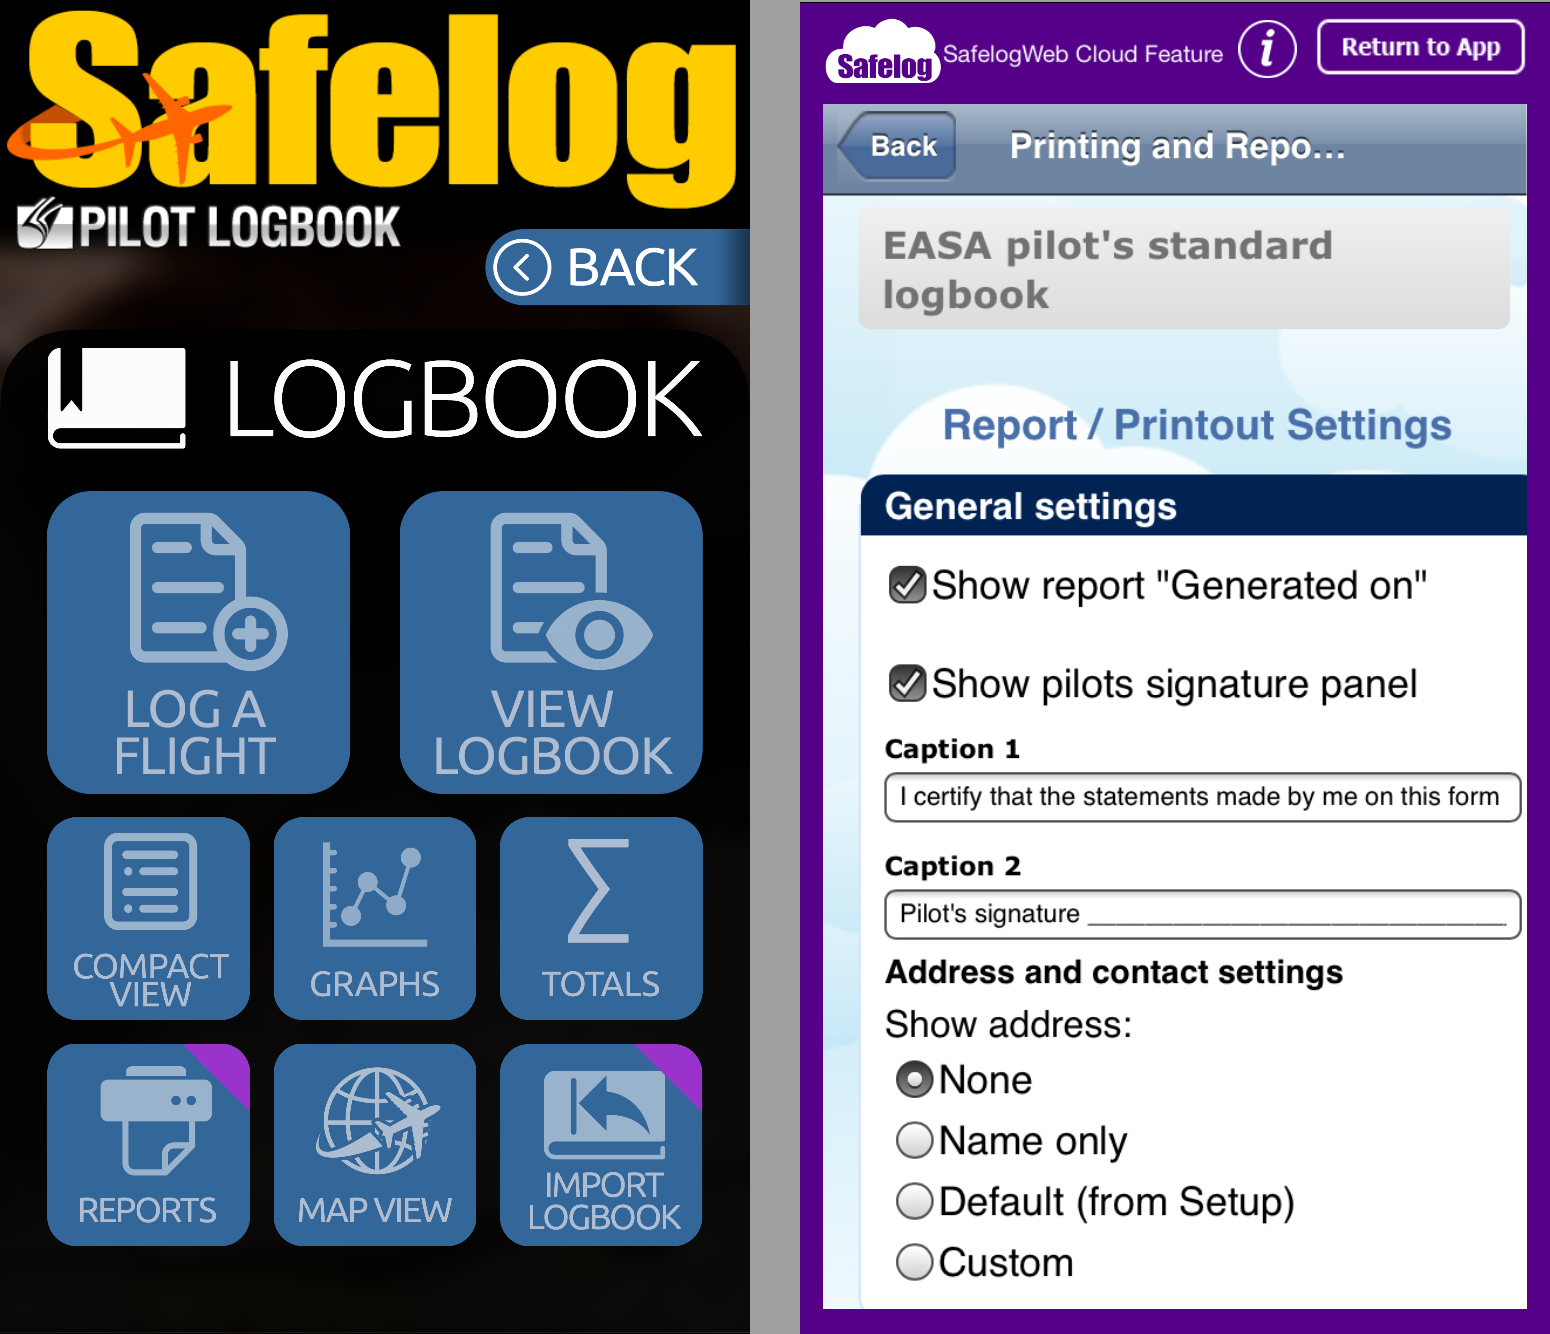
\includegraphics[width=0.99\textwidth]{./pictures/existujiciAplikace/Safelog}
 \caption[Safelog Pilot Logbook ]{Safelog Pilot Logbook }\label{fig:Safelog}
\end{figure}

\begin{figure}[]\centering
 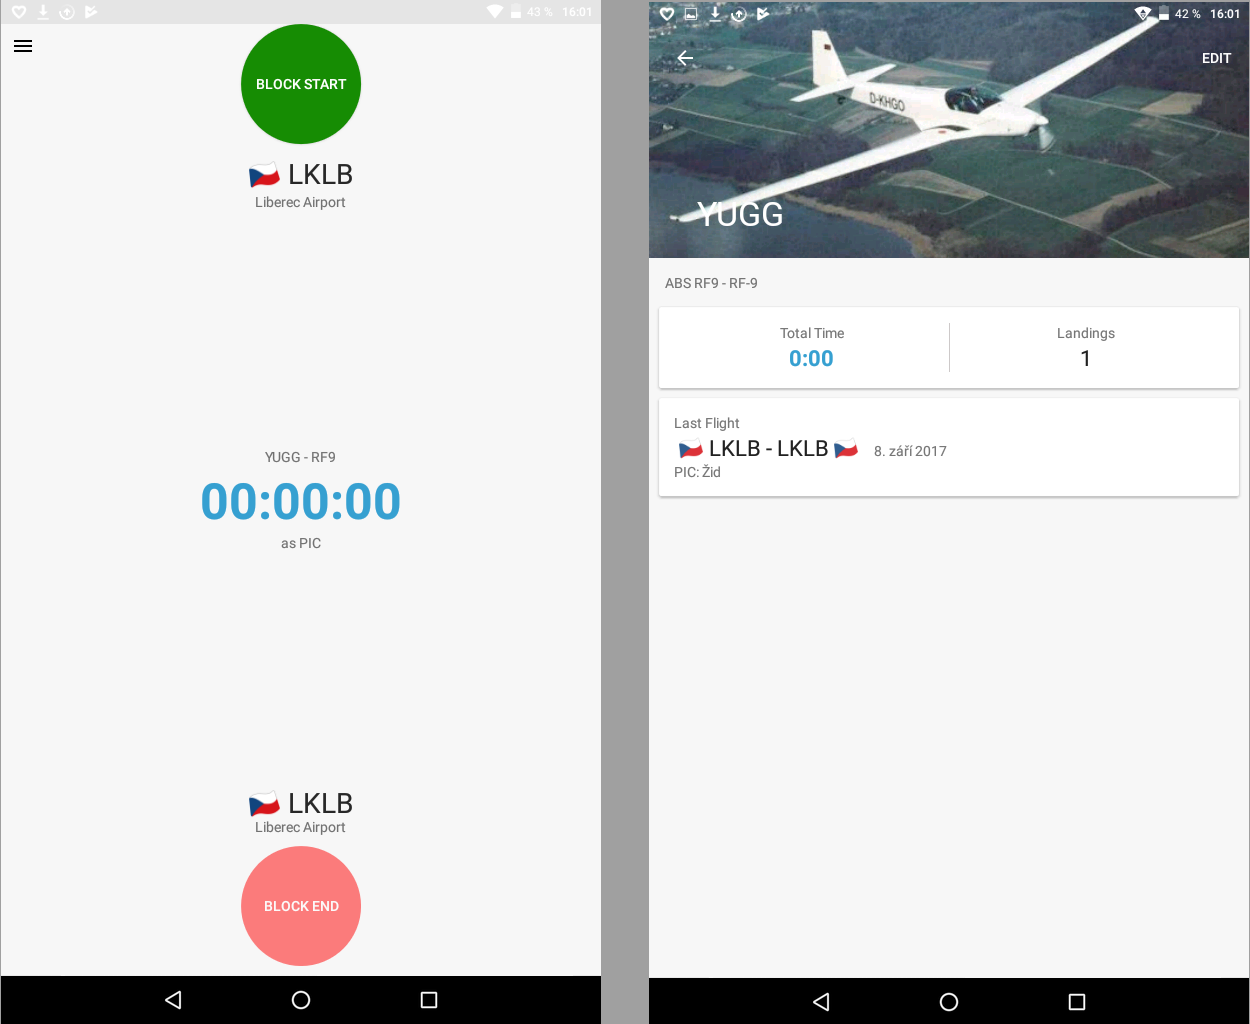
\includegraphics[width=0.99\textwidth]{./pictures/existujiciAplikace/FlyLogio}
 \caption[FlyLogio]{FlyLogio}\label{fig:FlyLogio}
\end{figure}

\begin{figure}[]\centering
 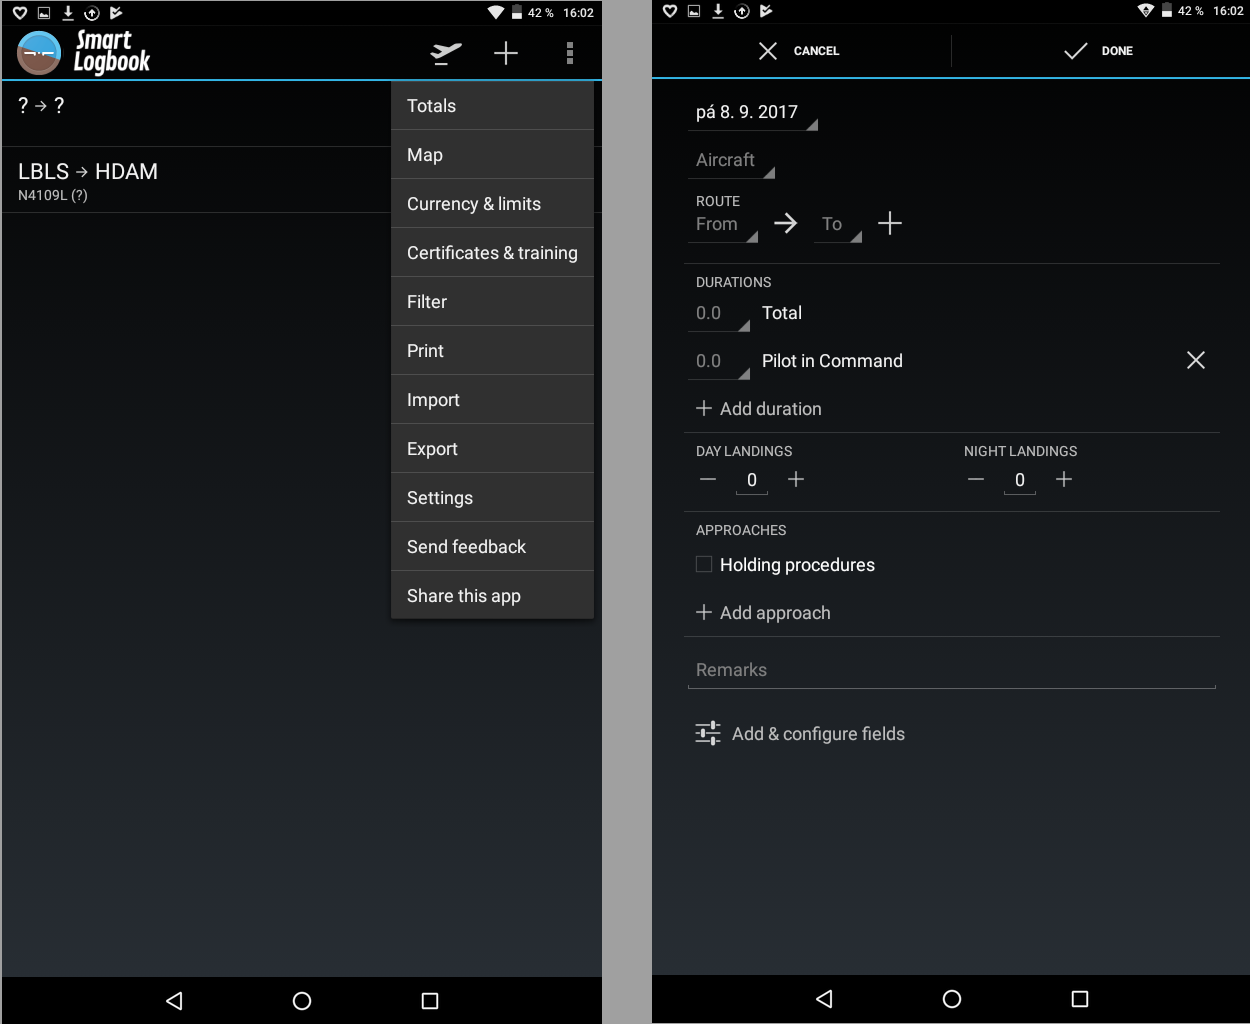
\includegraphics[width=0.99\textwidth]{./pictures/existujiciAplikace/SmartLogbook}
 \caption[Smart Logbook]{Smart Logbook}\label{fig:LogTenProX}
\end{figure}

\subsection{Kritéria hodnocení}
Kritéria hodnocení byla rozdělena do několika kategorií -- přihlášení, platby, napojení externích databází, doplňkové položky při vkládání záznamu, limity a certifikáty, reporty a zálohování.	

Při vkládání záznamu jsou brány v potaz pouze doplňkové položky, protože aplikace bude tvořena podle předpisu EASA FCL.050, který udává povinné údaje při evidování letu. Také položka v hodnocení  -- reporty podle EASA, je analyzována z pohledu předpisu FCL.050. 

Všechny položky hodnocení jsou uváděny z pohledu mobilní/tablet aplikace.

\subsection{Srovnávací tabulka}
\newcommand{\OK}{\ding{51}}
\newcommand{\NOK}{\ding{55}}
\newcommand{\rot}{\rotatebox{90}}

{\setlength\extrarowheight{2pt}
\begin{longtable}{@{\extracolsep{\fill}}l c c c c c c}
   \caption[Srovnávací tabulka]{Srovnávací tabulka}\label{tab:srovnavaci_tabulka} \\
   Kritéria & \rot{Log Ten Pro X} & \rot{Logbook Pro} & \rot{Safelog} &
   \rot{FlyLogio} & \rot{Smart Logbook} & \rot{Výsledek} \\
  \endfirsthead
   \caption[Srovnávací tabulka]{Srovnávací tabulka}\label{tab:srovnavaci_tabulka} \\
   Kritéria & \rot{Log Ten Pro X} & \rot{Logbook Pro} & \rot{Safelog} &
   \rot{FlyLogio} & \rot{Smart Logbook} & \rot{Výsledek} \\
  \endhead

   \hline
   \multicolumn{7}{c}{Přihlášení} \\
   \hline
   Aplikace funkční bez přihlášení 			 & \OK & \NOK & \NOK & \NOK & \NOK & 1/5 \\
   Možnost přihlášení								 & \OK & \OK & \OK & \OK & \OK  & 5/5 \\
   
   \hline
   \multicolumn{7}{c}{Platby} \\
   \hline
   Platby jednorázové			 & \NOK & \NOK & \NOK & \NOK & \OK & 1/5 \\
   Opakované platby			 & \OK & \OK & \OK & \OK & \OK  & 5/5 \\
   
   \hline
   \multicolumn{7}{c}{Napojení externích databází} \\
   \hline
   Napojení na databázi letišť		 & \NOK & \OK \footnote{Logbook Pro umí nalézt pouze nejbližší letiště.} & \OK & \OK & \OK & 4/5 \\
   Napojení na databázi letadel	 & \NOK & \NOK & \OK & \OK & \NOK  & 2/5 \\
   
   \hline
   \multicolumn{7}{c}{Doplňkové položky při vkládání záznamu} \\
   \hline
   Možnost přidání fotky						 & \OK & \NOK & \OK & \NOK & \NOK & 2/5 \\
   Možnost přidání dokumentu			 & \OK & \NOK & \OK & \NOK & \NOK & 2/5 \\
   
   \hline
   \multicolumn{7}{c}{Limity a certifikáty} \\
   \hline
   Kontrola limitů					 & \OK & \OK & \OK \footnote{Safelog zobrazuje limity ve webové verzi.} & \NOK & \OK & 4/5 \\
   Certifikáty							 & \OK & \OK & \OK \footnote{Safelog zobrazuje certifikáty ve webové verzi.} & \NOK & \OK & 4/5 \\
   
   \hline
   \multicolumn{7}{c}{Reporty} \\
   \hline
   Generování reportů					 & \OK & \NOK & \OK \footnote{Safelog zobrazuje reporty ve webové verzi.}  & \NOK & \OK & 3/5 \\
   Reporty podle EASA					 & \NOK & \NOK & \OK & \NOK & \OK & 2/5 \\
   Jiné reporty								 & \OK & \OK & \OK & \NOK & \OK & 2/5 \\
   
   \hline
   \multicolumn{7}{c}{Perzistence dat} \\
   \hline
   iCloud/Google					 & \OK & \NOK & \NOK & \OK & \OK & 3/5 \\
   Vlastní řešení						 & \NOK & \OK & \OK & \NOK & \NOK & 2/5 \\
   Synchronizace více zařízení  & \OK & \OK & \OK & \OK & \OK & 5/5 \\

\end{longtable}
}
\subsection{Výsledky a vlastní zhodnocení}
\subsubsection{LogTen Pro X}
LogTen Pro X je z analyzovaných iOS aplikací nejvíce uživatelsky přívětivá. Zobrazuje přehledně limity a certifikáty, i vkládání je intuitivní. Má však i několik nedostatků: 
\begin{itemize}
\item není napojená na databázi letišť, tudíž uživatel musí vyplnit všechny informace o daném letišti sám, bez automatického doplnění nebo našeptávání;
\item neumožňuje generování reportů podle předpisu EASA FCL.050;
\item aplikace je placená ročně --
	\begin{itemize}
	\item iPhone + iPad + Mac -- 3550 Kč,
	\item Mac -- 3550 Kč,
	\item iPhone + iPad -- 2150 Kč.
	\end{itemize}
\end{itemize}
Data o aplikaci a cenách jsou získány přímo z aplikace LogTen Pro X. 

\subsubsection{Logbook Pro Aviation Flight Log for Pilots}
Aplikace Logbook Pro vyžaduje pro přihlášení stažení PC aplikace (pouze pro Windows). S touto aplikací je následně synchronizován. Některá funkcionalita, např. generování reportů, je dostupná pouze v PC verzi.

PC verze aplikace je zadarmo pouze ve zkušební verzi, poté základní verze stojí v přepočtu 1800 Kč. iOS verze aplikace se platí ročně v přepočtu za 1045 Kč, je nutné si zaplatit i zálohování a další funkcionality. \cite{SafelogPrices}

\subsubsection{Safelog Pilot Logbook}
Safelog Pilot Logbook obsahuje pouze některé funkce přímo v aplikaci, u ostatních je uživatel odkázán do webového rozhraní (SafelogWeb Cloud) viz. \ref{fig:Safelog}. Toto webové rozhraní zobrazené v aplikaci však není přizpůsobené pro mobilní zařízení, často je zobrazena pouze část stránky a není možné např. vyplnit všechna pole formuláře.

Tato aplikace však, pokud budeme brát v potaz i funkce ve webovém rozhraní, obsahuje nejširší spektrum funkcionalit.

Samotná aplikace je zadarmo, ale pro plnou verzi aplikace je nutné předplatné. To se pohybuje od 1320 Kč za jeden rok až po 8990 Kč za deset let. Data o aplikaci a cenách jsou získány z aplikace Safelog Pilot Logbook.

\subsubsection{FlyLogio - Pilot Logbook}
Android aplikace FlyLogio - Pilot Logbook je jedinou aplikací kompletně zadarmo. Z uživatelského pohledu se jedná o přehlednou a jednoduchou aplikaci.  Však neobsahuje takovou funkcionalitu jako ostatní placené aplikace, např. chybí generování jakýchkoliv reportů nebo kontrolování limitů.

\subsubsection{Smart Logbook}
Smart Logbook je poslední analyzovanou aplikací, jedná se o Android aplikaci. Obsahuje mnoho funkcionalit -- generování reportů podle mnoha norem, zobrazení mapy se zaznamenáním jednotlivých letů, hlídání limitů i expirace certifikátů.

Tato aplikace je zadarmo pouze ve zkušební verzi, následně je nutné aplikaci zakoupit za 300 Kč. Je nutné také platit za zálohování a synchronizaci dat, a to buď 20 Kč za měsíc, nebo 120 Kč za rok. Informace o cenách jsou získány z aplikace Smart Logbook.

\subsubsection{Závěr analýzy}
Tato analýza posloužila při návrhu funkcionalit iOS aplikace ve formě případů užití, při návrhu uživatelského rozhraní a také při výběru vhodného nástroje na perzistenci dat.

\chapter{Návrh}

\section{Funkční a nefunkční požadavky}
\subsection{Funkční požadavky}
Funkční požadavky jsou uvedeny pouze jmenovitě. Podrobnější popis je uveden v podobě případů užití.
\begin{enumerate}
\item Evidování leteckých záznamů.
\item Vyhledávání v leteckých záznamech.
\item Kontrola limitů.
\item Evidence zdravotních certifikátů.
\item Zobrazení statistik.
\item Generování reportů do formátu PDF.
\end{enumerate}
\subsection{Nefunkční požadavky}
\begin{enumerate}
\item Funkční pro iOS 11 -- aplikace bude dostupná pro verzi operačního systému iOS 11.
\item Aplikace pro iPhone a iPad -- uživatelské rozhraní bude přizpůsobeno jak telefonům, tak tabletům.
\item Stejná data na více uživatelových zařízeních -- všechna data budou zálohována online a uživatel k nim bude mít přístup na všech zařízeních s iOS 11 pod svým účtem.
\item Dostupnost dat offline -- uživatel bude mít přistup ke všem dříve staženým/vytvořeným záznamům. Aplikaci bude možné používat i bez internetového připojení, k synchronizaci dojde až ve chvíli, kdy bude internetové připojení k dispozici.
\item Aplikace podle EASA -- aplikace se bude řídit předpisy EASA a to přesně: FCL.050 u evidence letů,  ORO.FTL.210 v případě limitů a Part-MED při evidenci zdravotních certifikátů.
\end{enumerate}

\section{Navržená funkcionalita v podobě případů užití}
Případy užití (use cases) byly využity při návrhu funkcionalit iOS aplikace. Jsou obsaženy přímo v práci z důvodu přehledného zobrazení navržených funkcionalit a možnosti dovysvětlení u některých z nich.

Diagram případů užití zobrazuje obrázek \ref{fig:UC}. Tento diagram společně se projektem Enterprise Architect je k nalezení v příloze této práce.

\begin{figure}[]\centering
 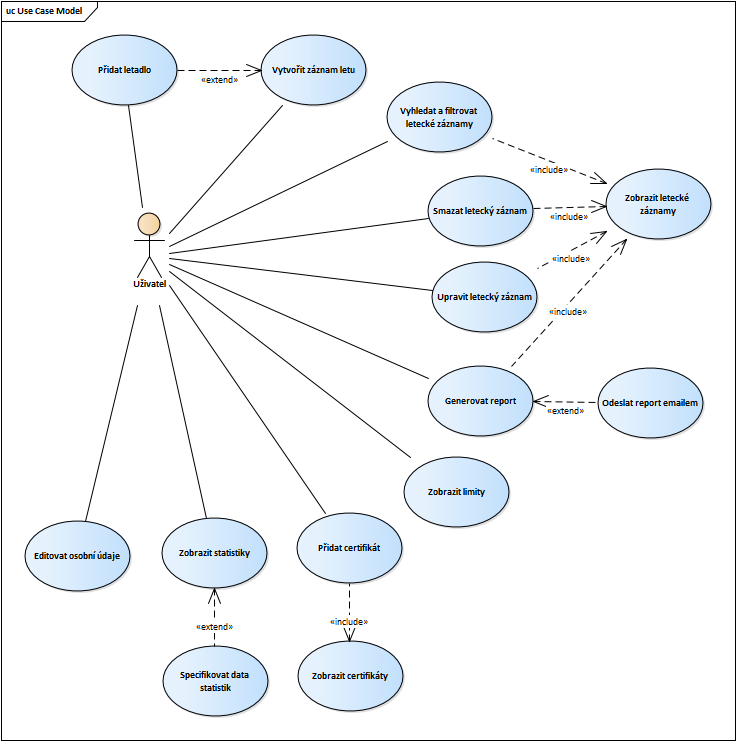
\includegraphics[width=0.99\textwidth]{./pictures/UC/UC}
 \caption[Případy užití]{Případy užití}\label{fig:UC}
\end{figure}

\subsection{Vytvořit záznam letu}
Vytvoření leteckého záznam umožňuje uživateli vložit nový záznam letu do aplikace.

Hlavní scénář --
\begin{itemize}
\item Případ užití začíná, když chce uživatel evidovat svůj let.
\item Systém zobrazí formulář umožňující zadat: jméno velícího pilota, datum letu, čas a místo odletu a příletu, letadlo, časy letu, celkový čas letu, počet vzletů a přistání, pilotovu funkci při letu a provozní podmínky.
\item Uživatel vyplní formulář.
\item Aplikace uloží informace o letu.
\end{itemize}

Alternativní scénář --
\begin{itemize}
\item Případ užití začíná, když chce uživatel evidovat záznam z výcvikového zařízení pro simulaci letu.
\item Systém zobrazí formulář umožňující zadat: typ a kvalifikační číslo výcvikového zařízení, datum a čas.
\item Případ užití pokračuje 3. krokem hlavního scénáře.
\end{itemize}

Aplikace nebude napojena na databázi letadel, protože uživatel u každého letadla musí vyplnit minimálně registrační číslo. Pokud by uživatel musel letadlo najít a zeditovat, je výhodnější pokud si sám letadlo přidá. Dalším důvodem k tomu rozhodnutí je, že pilot létá velmi často pouze s jedním letadlem a proto funkcionalitu přidání letadla nebude používat příliš často.

\subsection{Přidat letadlo}
Přidání letadla dává uživateli možnost přidat letadlo, které pak může vkládat do záznamů o letu.

\begin{itemize}
\item Případ užití začíná, když chce uživatel přidat nové letadlo.
\item Systém zobrazí formulář umožňující zadat: typ, značku model, variantu, registrační číslo letadla a zda je letadlo jednomotorové nebo vícemotorové.
\item Uživatel vyplní formulář.
\item Aplikace uloží letadlo.
\end{itemize}

\subsection{Zobrazit letecké záznamy}
Zobrazení leteckých záznamů zobrazuje jednotlivé záznamy v podobě tabulky, kde u každého záznamu jsou vidět základní informace. Mezi tyto informace patří: místo odletu a přílet, datum, čas letu a letadlo.

\subsection{Vyhledat a filtrovat letecké záznamy}
Tato funkcionalita umožňuje uživateli vyhledávání a filtrování leteckých záznamů.

\begin{itemize}
\item Případ užití začíná, pokud chce uživatel vyhledat nebo vyfiltrovat letecké záznamy.
\item Include(Zobrazit letecké záznamy).
\item Aplikace zobrazí formulář, který umožňuje: zadat hledaný text, nastavit zda se jedná o záznam letu nebo o záznam z výcvikového zařízení, zvolit typ letadla nebo přesné letadlo a nastavit období.
\item Uživatel vyplní pole, podle kterých chce vyhledávat/filtrovat.
\item Systém zobrazí pouze záznamy odpovídající zvoleným parametrům.
\end{itemize}

\subsection{Smazat letecký záznam}
Smazání leteckého záznamu umožňuje uživateli smazat letecký záznam, který předtím sám vytvořil.

\begin{itemize}
\item Případ užití začíná, když chce uživatel smazat jeden ze svých leteckých záznamů.
\item Include(Zobrazit letecké záznamy).
\item Uživatel si zvolí záznam, který chce smazat.
\item Aplikace zobrazí potvrzovací dialog.
\item Uživatel potvrdí smazání.
\item Aplikace odstraní položku ze seznamu.
\end{itemize}

\subsection{Upravit letecký záznam}
Upravení leteckého záznamu umožňuje uživateli upravit všechny položky zvoleného letecké záznamu.

\begin{itemize}
\item Případ užití začíná, když chce uživatel upravit letecký záznam.
\item Include(Zobrazit letecké záznamy).
\item Uživatel si zvolí záznam, který chce upravit.
\item Scénář pokračuje krokem 2 Vytvořit záznam letu.
\end{itemize}

\subsection{Zobrazit limity}
Tato funkcionalita slouží ke zobrazení limitů a kontrole zda jsou všechny limity v normě.

\subsection{Zobrazit certifikáty}
Tato funkcionalita umožňuje uživateli zobrazit všechny jeho certifikáty, společně s kontrolou platnosti a počtem dní do jejich expirace.

\subsection{Přidat certifikát}
Tato funkce umožňuje uživateli přidat certifikát a to buď dle šablony pro zdravotní certifikáty (LALP, třídy 1 a třídy 2), nebo vlastní.

\begin{itemize}
\item Případ užití začíná, když chce uživatel vytvořit nový certifikát.
\item Include(Zobrazit certifikáty).
\item Aplikace zobrazí formulář s možností vytvoření vlastního certifikátu nebo dle šablony. Ve formuláři je následně možné zadat: název certifikátu, datum vydání, datum expirace a popis.
\item Uživatel vyplní formulář.
\item Aplikace uloží certifikát.
\end{itemize}

\subsection{Zobrazit statistiky}
Zobrazení statistik zobrazuje nalétané hodiny (celkově, v noci, podle přístrojů a v různých pilotových funkcích).

\subsection{Specifikovat data statistik}
Tato funkcionalita umožňuje specifikovat data, ze kterých jsou zobrazeny statistiky.
Je možné specifikovat: text, zda jsou ve statistikách zobrazeny záznamy letů a/nebo záznamy ze simulátoru, typ letadla nebo přesné letadlo a období.

\subsection{Editovat osobní údaje}
Editace osobních údajů umožňuje uživateli upravit své osobní informace. Mezi tyto informace patří: jméno a příjmení, adresa a věk.

U osobních údajů je důležitý hlavně věk, který hraje roli u zdravotních certifikátů.

\subsection{Generovat report}
Generování reportu umožňuje uživateli vygenerovat report ve formátu PDF z nímž zvolených záznamů.

\begin{itemize}
\item Případ užití začíná, jestliže se uživatel rozhodne vygenerovat report.
\item Include(Zobrazit letecké záznamy).
\item Aplikace zobrazí náhled generovaného reportu.
\end{itemize}

\subsection{Odeslat report emailem}
Funkcionalita odeslání reportu emailem umožňuje uživateli, poté co vygeneroval report, odeslat tento report přes email.

\section{Návrh uživatelského rozhraní}
Návrh uživatelského rozhraní přímo navazuje na návrh funkcionalit. Pro tento návrh byl použit wireframe.

\subsection{Wireframe}
Wireframe je technika, která se používá v brzké fázi vývoje softwaru \cite{nngWireframe} pro rozvržení základních prvků obrazovek a navržení hlavních průchodů aplikací (navigace). Protože se jedná pouze o návrh, nemusí wireframe podporovat dynamicky měnící se obsah nebo např. nemusí zobrazovat chybové hlášky.

Wireframe může posloužit k první heuristické analýze a k uživatelským testům ještě před vývojem dané aplikace. \cite{exux}

Wireframe byl pro tuto práci vytvořen ve webovém nástroji NinjaMock (\url{https://ninjamock.com}). Z tohoto nástroje byl wireframe následně exportován do formátu pdf a ninjamock package. Tyto exporty jsou k nalezení v příloze této diplomové práce. 

Exportovaný wireframe ve formátu pdf je uložený vždy ve dvou provedeních: se zobrazeným mobilním zařízením a bez něj, je tomu tak, protože ve verzi se zobrazeným mobilním zařízením u obrazovek s více položkami (např. přidání záznamu letu) nejsou všechny položky vidět. U provedení bez zobrazeného mobilního zařízení jsou vždy všechny položky vidět, ale wireframe působí neúplným dojmem. Pro úplnost je přidána verze ninjamock package, kterou je možné importovat do webového nástroje NinjaMock. V této verzi jsou funkční i odkazy mezi jednotlivými obrazovkami. 

\subsection{Heuristická analýza}
Heuristická analýze je metoda, která se používá pro hledání problémů použitelnosti (usability problems) v uživatelském rozhraní. \cite{howtoheuristic} Jakob Nielsen vytvořil deset základních principů pro uživatelské rozhraní --
\begin{enumerate}
 \item \uv{viditelnost stavu systému,
 \item spojení systému a reálného světa,
 \item uživatelská kontrola a volnost,
 \item konzistence a standardizace,
 \item předcházení chyb,
 \item rozpoznání místo vzpomínání,
 \item flexibilita a efektivita použití,
 \item estetika a minimalismus,
 \item pomoci uživatelům rozpoznat, pochopit a vzpamatovat se z~chyb,
 \item nápověda a dokumentace} \cite{10heuristics} (překlad vlastní).
\end{enumerate}

Tato pravidla byla použita při heuristické analýze vytvořeného wireframu. Však nebyla kontrolována pravidla:
\begin{itemize}
\item \uv{předcházení chyb} -- z důvodu, že ve fázi návrhu není možné např. vyplnit formulář a nebo smazat záznam letu;
\item \uv{pomoci uživatelům rozpoznat, pochopit a vzpamatovat se z~chyb} -- také není možné vyvolat chybu;
\item \uv{nápověda a dokumentace}.
\end{itemize}

Článek Jakoba Nielsena \cite{howtoheuristic} doporučuje více hodnotitelů, kteří provedou nezávisle heuristickou analýzu nad daným návrhem uživatelského rozhraní. Počet nalezených problémů v závislosti na počtu hodnotitelů zobrazuje obrázek \ref{fig:heur}. Z grafu je možné usuzovat vhodný počet hodnotitelů pět až šest. Protože se však nyní jedná pouze o návrh, kde není možné testovat všechna pravidla, byli použiti pouze dva hodnotitelé.

\begin{figure}[h]\centering
 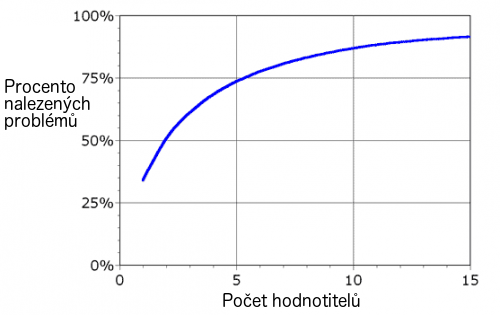
\includegraphics[width=0.99\textwidth]{./pictures/heur_eval_finding_curve_trans}
 \caption[Počet nalezených problémů v závislosti na počtu hodnotitelů]{Počet nalezených problémů v závislosti na počtu hodnotitelů. \cite{heur-eval-curve} (překlad vlastní)}\label{fig:heur}
\end{figure}

Po provedení heuristické analýzy byla vytvořena tabulka \ref{tab:heuristics} zobrazující nalezené problémy společně s jejich řešením a ohodnocením 1--5, kde číslo 1 identifikuje pouze drobný problém a číslo 5 velice závažný problém. Byla také vytvořena nová verze wireframe, která je také k nalezení v příloze této práce.

\begin{table}
\begin{tabular}{ c | c | p{9cm} }
Pravidlo & Závažnost & Provedená úprava \\
\hline
1 & 3 & Při přidávání nového záznamu se bude měnit nadpis (title) podle toho zda je přidáván záznam o letu nebo ze simulátoru. \\
2 & 2 & Tlačítko \uv{Zavřít} bude přejmenováno na \uv{Zrušit}. Tato změna se týká obrazovek -- přidat záznam, přidat letadlo a přidat certifikát.\\
2 & 3 & U nastavení hledání bude tlačítko \uv{Zpět} přejmenováno na \uv{Zrušit}.\\
2 & 4 & Přejmenování záložky \uv{Nastavení} na \uv{Profil} a změnění ikonky.\\
2 & 4 & Přejmenování \uv{Můj profil} (v bývalé záložce \uv{Nastavení}) na \uv{Osobní informace}.\\
2 & 2 & Doplnění \uv{Certifikáty} na \uv{Zdravotní certifikáty}.\\
8 & 2 & U zobrazení všech záznamů jsou zredukovány zobrazené informace na datum, čas, místo a letadlo. \\
\end{tabular}
\caption[Nalezené problémy použitelnosti]{Nalezené problémy použitelnosti}\label{tab:heuristics}
\end{table}

\subsection{Uživatelské testy}
Uživatelské testy byly provedeny po heuristické analýze (na upraveném wireframu) ještě před samotnou implementací. Testy také nebylo možné provést v plné míře a sloužili převážné k odhalení nejvíce problematických částí návrhu uživatelského rozhraní.

Jakob Nielsen \cite{usabilityTestingNNG} doporučuje pět uživatelů na uživatelské testování. Však ze stejných důvodů jako u heuristické analýzy, byly zvoleni nyní pouze dva uživatelé.

Rozsáhlejší testování a heuristická analýza bude provedeno až po dokončení prototypu aplikace.

Testovaní uživatelé nebyly děleni v této fázi do skupin z důvodu jejich malého počtu. Podmínky na uživatele však kladeny byly -- oba uživatelé museli používat operační systém iOS minimálně po dobu jednoho rok a alespoň jeden z nich se musel pohybovat v leteckém průmyslu.

Pro oba uživatele byly vytvořeny stejné testovací scénáře. Uživateli, který neměl znalosti z letectví, byly nejprve vysvětleny základní pojmy nutné k absolvování scénářů a až poté bylo provedeno testování.

\subsubsection{Scénáře}
\begin{enumerate}
\item Právě jste dokončil(a) svůj první let z Brna do Prahy. Z Brna jste odlétal(a) v 7:00 a do Prahy jste přiletěl(a) v 8:45, neměl jste žádné mezipřistání. Celou doby jste zastával(a) funkci vedoucího pilota a letěl(a) jste letadlem Boeing. Zaznamenejte svůj let.
\item Zjistil(a) jste, že jste u minulého záznamu chybně zaznamenal(a) čas. Upravte tedy čas příletu do Prahy na 7:45.
\item Chcete si přidat další záznam, tentokrát z výcvikového zařízení. Zadejte dnešní datum, čas na zařízení dvě hodiny a znovu jste zastával(a) funkci vedoucího pilota.
\item Aplikaci používáte již delší dobu a máte tedy i více záznamu. Zobrazte si pouze lety, které byly provedeny za poslední týden.
\item Jeden ze záznamů z minulého kroku smažte.
\item Zobrazte si svůj profil a zkontrolujte, zda jsou všechny položky vyplněny správně. Pokud ne, opravte chybně vyplněné nebo chybějící pole.
\item U letadla Boeing z prvního kroku chcete změnit model. Proveďte tuto úpravu.
\item Za poslední tři týdny jste absolvoval(a) mnoho letů, zkontrolujte, zda jste nepřekročil jeden z limitů.
\item Dnes Vám vydali zdravotní certifikát třídy jedna (Class 1). Vložte ho do aplikace.
\item Vytvořte report ze všech záznamů letů i záznamů z výcvikového zařízení za posledních čtrnáct dní.
\end{enumerate}

\subsubsection{Výsledky testů a provedené úpravy}
Testovaní uživatelé byli při jednotlivých testech pozorováni, aby bylo zjištěno co a proč dělají špatně. Z čehož byly následně vyvozeny nutné úpravy v uživatelském rozhraní.

\begin{enumerate}
\item Smazání záznamu budu možné nyní ještě u detailu tohoto záznamu. Tato funkcionalita bude ještě znovu podrobena testu u prototypu aplikace. Gesto $swipe$ se u wireframu špatně testuje.
\item \uv{Má letadla} již nebudou pod záložkou \uv{Profil}, ale budou představovat samostatný $tab$.
\item Vytvoření reportu bude nyní označeno ještě navíc textem.
\item Při přidávání nového záznamu si uživatel nejprve vybere zda se jedná o záznam letu nebo o záznam ze simulátoru.
\item U zobrazení seznamu záznamů budou informace o jednotlivých záznamech v jiném pořadí -- datum, čas, místa vzletu a příletu a letadlo.
\end{enumerate}

Po provedení testování s pilotem byla diskutována navržená funkcionalita. Výsledkem této diskuze bylo:
\begin{itemize}
\item přidání celkové statistiky nalétaných hodin,
\item filtrování bude nyní možné i podle typu letadla,
\item záznamy letů budou zobrazovat nyní registrační číslo letadla místo jeho modelu, typu a varianty.
\end{itemize}

Případy užití zobrazené v této práci již zahrnují tuto přidanou a upravenou funkcionalitu. Po uživatelských testech a diskuzi byla vytvořena i poslední verze wireframe, také k nalezení v příloze této diplomové práce.

\section{Navržená řešení pro tvorbu aplikace}
Tato kapitola popisuje a zdůvodňuje zvolená řešení architektury, perzistence dat a FRP framework.

\subsection{Architektura}
Pro svou práci jsem si na základě navržených funkcionalit zvolil architekturu MVVM. Architektura MVVM eliminuje nevýhodu MVC -- příliš mnoho logiky a kódu ve vrstvě $Controller$, a na druhou stranu není zbytečně složitá (pro navrženou funkcionalitu) jako VIPER.

\subsection{Perzistence dat}
Pro tvorbu aplikace na evidenci letů jsem si zvolil možnost perzistence dat pomocí Realmu. Prvním z důvodů této volby je podpora online i offline uložení dat. To umožňuje uživateli mít stejná data na více zařízeních, však i společně s možností používat aplikaci offline. Dalším důvodem bylo to, že je Realm zcela zdarma, což mu dává výhodu oproti iCloud -- Apple řešení.

\subsection{FRP framework}
Pro realizaci aplikace byla zvolena ReactiveCocoa jako FRP framework. ReactiveCocoa byla vybrána, protože příhodně rozšiřuje framework ReactiveSwift, má také přehlednou dokumentaci a existují kvalitní příklady demonstrující použití tohoto frameworku.

\chapter{Realizace}
\label{chap:realizace}

\section{Programovací jazyk Swift}
Swift je programovací jazyk vytvořený společností Apple. Jedná se o nástupce jazyku C a Objective-C a používá se pro tvorbu iOS, macOS, watchOS a tvOS aplikací.

Swift je objektově orientovaný open source jazyk. Mezi jeho hlavní přednosti patří: 
\begin{itemize}
\item automaticky spravovaná paměť,
\item podpora i funkcionálního programování (filter, map, reduce),
\item možnost vracení  více  hodnot z funkcí,
\item podpora tzv. generics,
\item nativní zpracovávání chyb pomocí try, cache, trow,
\item podpora protokolů a tzv. extension (rozšíření již existujících tříd). \cite{swift}
\end{itemize}

Swift je relativně mladý programovací jazyk, první oznámení proběhlo roku 2014 a nyní je nejnovější verzí Swift 4. Právě v této verzi byla implementována aplikace v rámci této diplomové práce. \cite{swift2}

V této kapitole jsou dále rozebírány některé funkcionality a vlastnosti jazyka Swift společně s ukázkami kódu z vytvářené aplikace.

\subsection{Optionals}
Swift je tzv. typově bezpečný jazyk, což zaručuje to, že daná proměnná bude mít vždy stejný typ. Tedy např. pokud náš kód vyžaduje $String$ není možné zadat $Int$. 
Proměnné se definují klíčovým slovem $var$ a konstanty $let$. Proměnné musí být vždy inicializované před použitím a objekty nikdy nemohou být $nil$. Pro práci s hodnotami $nil$ jsou ve Swiftu zavedeny tzv. $Optinals$.

$Optinal$ je jakýsi obal (wrapper) klasických typů ($String$, $Int$, $Double$ apod.), který reprezentuje dvě možnosti: hodnota je nastavena a je tedy možné tzv. $unwrap$ $optinal$ a tím získat danou hodnotu, nebo hodnota není nastavena (jedná se o $nil$). \cite{devBasics}

Příklad \ref{lst:optinal} zobrazuje nejprve inicializaci $optional$ proměnné, kde otazník indikuje $optinal$ hodnotu uvnitř proměnné. Následně je ve funkci $save$ použito pro $unwrap$ proměnné tzv. $optional$ $binding$. To zpřístupní hodnotu $optional$ proměnné (pokud byla hodnota nastavena) v podobě dočasné konstanty. V případě, že je hodnota předána dočasné proměnné, můžeme k ní přistupovat klasicky a v našem případě delegovat funkci $save$.

\begin{figure}
\begin{minipage}{\linewidth}
\begin{lstlisting}[caption={Příklad práce s Optinal},label={lst:optinal}]
// optinal variable initialization
var delegate: NoteViewControllerDelegate? = nil
...
private func save(note: String) {
   // optional variable unwarpping using optional binding
   if let unwappedDelegate = delegate {
      unwappedDelegate.save(note: note)
   }
   ...
}

\end{lstlisting}
\end{minipage}
\end{figure}


\subsection{Extensions}
Extension, neboli rozšíření, je klíčové slovo v jazyce Swift, které umožňuje přidat novou funkcionalitu nebo atributy k již existující třídě, struktuře, protokolu apod. Toto zahrnuje i třídy, u kterých není možné upravit jejich zdrojový kód, tedy např. třídy UIKit.

Extensions umožňují: 
\begin{itemize}
	\item definovat nové metody,
	\item přidat konstruktory, 
	\item upravit typ tak, aby splňoval daný protokol a další. \cite{devExtensions}
\end{itemize}

Ukázka \ref{lst:extension} předvádí rozšíření třídy $UITableViewController$ o novou generickou metodu. Tato metoda je použita u dynamických tabulek zobrazujících data z Realmu. Díky principů FRP může tabulka jednoduše podporovat např. smazání záznamu, protože je neustále pozorován $Signal$ se změnami a podle změn jsou následně provedeny vhodné animace na straně $UITableView$.

Dalšího klíčového slova, kterého je možné si v ukázce všimnout je $guard$. $Guard$ je možné vnímat podobně jako tzv. assert. Tedy zadáváme podmínku, u které chceme aby byla splněna, pokud splněna není dostáváme se do povinné $else$ větve. Klíčové slovo $guard$ je jednou z možností pro $unwrap$ $optional$ proměnné a také zamezuje několikanásobné podmínce $if-else$ (ve složitějších případech), čímž dochází k zpřehlednění kódu. \cite{devGuard}

\begin{figure}
\begin{minipage}{\linewidth}
\begin{lstlisting}[caption={Ukázka Extension},label={lst:extension}]
extension UITableViewController {
    func observeSignalForTableDataChanges<T>(
      with signal: Signal<RealmCollectionChange<Results<T>>,
      NoError>) {
      // observing input signal
      signal.observeValues{ [weak self] changes in
         guard let tableView = self?.tableView
            else { return }
         // switch on changes type   
         switch changes {
         case .initial:
            tableView.reloadData()
         case .update(_, let deletions, let insertions,
                     let modifications):
            tableView.beginUpdates()
            tableView.insertRows(at: insertions.map
               ({ IndexPath(row: $0, section: 0) }),
               with: .automatic)
            tableView.deleteRows(at: deletions.map
               ({ IndexPath(row: $0, section: 0)}),
               with: .automatic)
            tableView.reloadRows(at: modifications.map
               ({ IndexPath(row: $0, section: 0) }),
               with: .automatic)
            tableView.endUpdates()
         case .error(let error):
            fatalError("\(error)")
         }
      }
   }
}
\end{lstlisting}
\end{minipage}
\end{figure}
	
\subsection{Protokoly}
Protokoly představují ve Swiftu předpis metod, vlastností a dalších náležitostí, které jsou nutné pro splnění daných úloh. Podmínky protokolu mohou splňovat třídy, struktury a další tím, že poskytnou implementaci všech požadavků. \cite{devProtocol}

V rámci implementace aplikace bylo definováno několik protokolů. Například v ukázce \ref{lst:optinal}, musel $delegate$ odpovídat protokolu\\ $NoteViewControllerDelegate$ a tedy mít implementovanou metodu $save$ (ukázka definování protokolu viz. \ref{lst:protocol}). Jak je možné vidět, protokol neurčuje jak má být metoda implementována, pouze určuje její definici.

Princip delegování je v jazyce Swift velice častý. I mnoho tříd např. z UIKit vyžaduje pro podporu určitých funkcionalit splnění daného protokolu. Ukázka \ref{lst:pickerdelegate} ukazuje implementaci protokolu $UIPickerViewDelegate$\\ a $UIPickerViewDataSource$. Kdy po implementaci příslušných metod a nastavení $UITableViewController$ jako delegáta, je možné ve $View$ pracovat s komponentou $UIPickerView$.
	
\begin{figure}
\begin{minipage}{\linewidth}
\begin{lstlisting}[caption={Definice protokolu},label={lst:protocol}]
protocol NoteViewControllerDelegate {
   func save(note: String)
}
\end{lstlisting}
\end{minipage}
\end{figure}	

\begin{figure}
\begin{minipage}{\linewidth}
\begin{lstlisting}[caption={Implementace protokolu},label={lst:pickerdelegate}]
class AddMedicalCertificateViewController: 
RecordTableViewController, 
UIPickerViewDelegate, 
UIPickerViewDataSource {

   private let picker = UIPickerView()

   override func viewDidLoad() {
      // setting self as delegate
      picker.delegate = self
   }

   // MARK: - UIPickerViewDataSource

   func numberOfComponents(in pickerView: UIPickerView) 
       -> Int {
      return 1
   }

   func pickerView(_ pickerView: UIPickerView, 
         numberOfRowsInComponent component: Int) -> Int {
      return viewModel.getTypesCount()
   }

   func pickerView(_ pickerView: UIPickerView, 
         titleForRow row: Int, forComponent component: Int)
       -> String? {
      return viewModel.getType(for: row)
   }

   func pickerView(_ pickerView: UIPickerView, 
         didSelectRow row: Int, 
         inComponent component: Int) {
      typeTextField.text = viewModel.getType(for: row)
      viewModel.typeString.value = 
         viewModel.getType(for: row)
   }
}
\end{lstlisting}
\end{minipage}
\end{figure}	
	
\subsection{Automatické počítání referencí}
Automatická správa paměti, jak už je řečeno dříve, je jednou z předností Swiftu. Tato správa je zajištěna metodou automatického počítání referencí. Toto počítání zajišťuje udržení reference dané instance pouze po dobu, co je opravdu potřebná. V době, kdy instanci není nutné udržovat (již neexistují žádné reference), dojde k uvolnění předem alokované paměti.

Swift definuje tři druhy referencí -- $strong$, $weak$ a $unowned$. Nejčastějším a základním případem je $strong$ reference, které zaručuje, že instance, na kterou reference ukazuje, nebude dealokována dokud reference existuje. Může však nastat případ nazývaný cyklus $strong$ referencí, který způsobí tzv. paměťový $leak$ (nedojde k uvolnění veškeré alokované paměti). Tento cyklus může být způsoben vzájemnými referencemi dvou instancí nebo např. pokud třídní $closure$ zachytí $self$. Z tohoto důvodu jsou vytvořeny další dva typy referencí. $Weak$ reference neudržuje $strong$ referenci na instanci a není tedy bráněno dealokaci dané instance. Toto chování umožňuje i to, že $weak$ reference může mít hodnotu $nil$. $Weak$ reference se používá pokud má instance v referenci kratší životnost než samotná instance vlastnící referenci. $Unowned$ reference se používá v opačném případě a nemůže mít nikdy hodnotu $nil$. \cite{devMemory}

\subsection{Použíté Apple frameworky}
Aplikace využívá třech Apple frameworků -- UIKit, Foundation a CloudKit.

UIKit je základním frameworkem pro $View$ část aplikace. Obsahuje části pro:
\begin{itemize}
\item vytvoření uživatelského rozhraní;
\item zajištění komunikaci mezi uživatelem, systémem a aplikací;
\item zpracování uživatelských interakcí;
\item kreslení a tisknutí;
\item animace a mnohé další. \cite{UIKit}
\end{itemize} 

Foundation obsahuje základní datové typy, kolekce, třídy atd. Umožňuje i perzistenci dat, práci s datem a časem nebo poskytuje funkce pro práci s textem. \cite{foundation}

CloudKit framework umožňuje práci s iCloudem, tedy ukládání dat a přístup k k uloženým datům z více zařízení. V této aplikaci byl tento framework použit pouze pro autentizaci uživatele (dále popsáno v kapitole: \nameref{chap:login}).

\section{Reactive Cocoa}
Tato kapitola se zabývá jednotlivými prvky frameworků Reactive Cocoa a Reactive Swift, společně s ukázkami a vysvětlením jak byly v aplikaci použity. Na ukázkách je také znázorněno, jak principy FRP fungovaly s MVVM architekturou.

\subsection{Signal}
Prvním základním prvkem frameworku Reactive Swift je $Signal$. Jedná se datový tok, který posílá v průběhu svého života události (Events) -- hodnoty (Value) nebo chyby (Error). Všichni pozorovatelé daného $Signalu$ dostávají stejné události ve stejný čas a nejsou schopni $Signal$ svou činností ovlivnit. \cite{signal}

Příklad \ref{lst:signal} zobrazuje použití prvku $Signal$. Společně se $Signalem$ je vytvořen ještě $Observer$. Tato dvojice je vytvořena pomocí funkce $pipe$, která vrací společně navázanou dvojici $Signal$ a $Observer$. Tato dvojice následně pracuje spolu -- všechny události odeslané $Observeru$ jsou možné pozorovat na $Signalu$. $Signal$ zobrazený v ukázce se stará o informování o změnách v kolekci Realm objektů. Tento druh $Signalu$ je ten, který následně zpracovává příslušný $UITableViewController$ pomocí rozšíření (extension) zobrazené na příkladu \ref{lst:extension}.

\begin{figure}
\begin{minipage}{\linewidth}
\begin{lstlisting}[caption={Ukázka použití prvku Signal},label={lst:signal}]
class RealmTableViewModel<T: Object>: RealmViewModel {
   ...
   // observed collection (using Realm notifications)
   internal var collection: Results<T>?
   let collectionChangedSignal: 
      Signal<RealmCollectionChange<Results<T>>, NoError>
   private let collectionChangedObserver: Signal
      <RealmCollectionChange<Results<T>>, NoError>.Observer

   override init() {
      // signal and observer initialization
      let (arrayChangedSignal, arrayChangedObserver) = 
         Signal<RealmCollectionChange<Results<T>>, NoError>
         .pipe()
      self.collectionChangedSignal = arrayChangedSignal
      self.collectionChangedObserver = arrayChangedObserver
      super.init()
   }
    ...
   internal func collectionChangedNotificationBlock(
      changes: RealmCollectionChange<Results<T>>) {
      collectionChangedObserver.send(value: changes)
   }
}
\end{lstlisting}
\end{minipage}
\end{figure}	

\subsection{SignalProducer}
Dalším prvkem je $SignalProducer$. $SignalProducer$ vytváří $Signal$ a je využíván společně s $Action$. $Signal$ je vytvářen pomocí funkce $start()$. Tato funkce vytvoří vždy nový $Signal$ a z toho důvodu různé $Signaly$ mohou mít různé verze událostí nebo se mohou úplně lišit. \cite{signalProducer}

$SignalProducer$ je zobrazen v ukázce \ref{lst:action} společně s prvkem $Action$.

\subsection{MutableProperty}
$MutableProperty$ je dalším prvkem frameworku Reactive Swift. $MutableProperty$ obsahuje hodnotu, u které je možné pozorovat její změny. Tento prvek také obsahuje vlastní prvky typu $Signal$ a $SignalProducer$. \cite{property}

$MutableProperty$ v aplikaci představuje nejčastější způsob namapování $View$ na $ViewModel$. Ukázka \ref{lst:property} zobrazuje hned několik propojení jednotlivých vrstev architektury. První propojení přestavuje proměnná $fromTextField$, která je označená jako $@IBOutlet$. Právě toto označení se používá při spojení prvků $storyboardu$ s kódem. Další propojení, tentokrát již vrstev $View$ a $ViewModel$, je zobrazeno ve funkci $bindViewModel$, kde dojde nejprve k nastavení výchozí hodnoty pole $UITextField$ a následně jsou pozorovány všechny změny. Toto pozorování umožňuje framework Reactive Cocoa, který přidává UI prvkům vlastnost $reactive$.

Při nastavování výchozí hodnoty $UITextFieldu$ závisí na tom zda se jedná o vytváření nového záznamu letu nebo o úpravu již existujícího. Podle toho je vytvořen $ViewModel$ (se záznamem letu nebo s hodnotou $nil$) i $MutableProperty$.

\begin{figure}
\begin{minipage}{\linewidth}
\begin{lstlisting}[caption={Ukázka propojení $View$ a $ViewModel$},label={lst:property}]
// View
class AddFlightRecordTableViewController: 
RecordTableViewController {
   // storyboard reference
   @IBOutlet weak var fromTextField: UITextField!

   override func viewDidLoad() {
      super.viewDidLoad()
      ...
      bindViewModel()
   }

   private func bindViewModel() {
      // setting default value
      fromTextField.text = viewModel.from.value
      // bind UITextField to MutableProperty
      viewModel.from <~ toTextField.reactive
         .continuousTextValues.filterMap{ $0 }
      ...
   }
}

// ViewModel
class AddFlightRecordViewModel: RealmViewModel {
   let from: MutableProperty<String?>
   ...
   init(with record: Record?) {
      from = MutableProperty(record?.from ?? nil)
      ...
   }
}
\end{lstlisting}
\end{minipage}
\end{figure}	

\subsection{Action}
$Action$ je posledním použitým prvkem frameworku Reactive Swift. Hlavní částí prvku $Action$ je tzv. $execute$ reprezentovaný $SignalProducerem$. Tento $execute$ je zadán ve formě closure. $Action$ může obsahovat podmínku $enabledIf$, která určuje zda je umožněno akci provést.

Použití prvku $Action$ je zobrazeno v ukázce \ref{lst:action}. Akce je znovu napojena pomocí vlastnosti $reactive$ frameworku Reactive Cocoa. Samotná akce pouze odesílá na stisknutí tlačítka proměnnou $note$, která je následně delegována do jiného $Controlleru$. Tato akce je však proveditelná pouze pokud je splněna podmínka v části $enabledIf$, tedy $note$ nemá nulovou délku. Díky propojení s tlačítkem ve $View$ se proveditelnost akce promítá i do vlastností tlačítka $UIBarButtonItem$. Po provedení akce je informován $observer$ ve $View$, který pozoruje $Signal$ vytvářený $SignalProducerem$ akce.

\begin{figure}
\begin{minipage}{\linewidth}
\begin{lstlisting}[caption={Ukázka použití Action},label={lst:action}]
// View
class NoteViewController: UIViewController {
   @IBOutlet weak var saveBtn: UIBarButtonItem!
   ...
   override func viewDidLoad() {
      super.viewDidLoad()
      ...
      bindViewModel()
   }
   
   private func bindViewModel() {
      // binding action to button
      saveBtn.reactive.pressed = 
         CocoaAction(viewModel.saveAction)
      // observing action values
      viewModel.saveAction.values.observeValues(save)
      ...
   }  
} 

// ViewModel
class NoteViewModel {
   var note: MutableProperty<String?>
   let saveAction: Action<(), String, NoError>
   
   init(note: String?) {
      self.note = MutableProperty(note)
      // action definition
      saveAction = Action<(), String, NoError>(
         state: self.note, enabledIf: {
         if let note = $0 {
            return note.count > 0
         }
         return false
      }) { note, _ in
         return SignalProducer<String, NoError> { 
            observer, _ in
            observer.send(value: note!)
         }
      }
   }
}
\end{lstlisting}
\end{minipage}
\end{figure}	

\subsection{Použité základní operátory}
Reactive Swift obsahuje mnoho operátorů, které umí nějakým způsobem upravovat pozorované toky dat. Tato kapitola se zabývá jednotlivými použitými operátory společně s ukázkami jejich použití v aplikaci.

\subsubsection{Map}
Operátor $map$ je jeden z nejzákladnějších operátorů funkcionálního programování. V případě Reactive Swift přetváří hodnoty jednoho datového toku na jiný datový tok. \cite{operators}

V aplikaci byl operátor $map$ velice užitečný. Byl použit hlavně pro spojení dvou $MutableProperty$ s odlišnými typy. Toto spojení probíhalo např. při práci s $UIDatePicker$ (výběr datu), kdy jedna $MutableProperty$ získává uživatelovi vstupy ve formátu $Date$ a tento tok hodnot je průběžné transformován jako $String$ do druhé $MutableProperty$. Ukázka je zobrazena v kódu \ref{lst:map}. V ukázce je možné vidět, že přepis transformace je zadán jako již existující funkce, stejného výsledku je však možné dosáhnout i při zadání přepisu ve formě closure.

\begin{figure}
\begin{minipage}{\linewidth}
\begin{lstlisting}[caption={Ukázka použití Map},label={lst:map}]
extension DateFormatter {
   struct Format {
       static let date = "dd.MM.yyyy"
   }
   func dateToString(from date: Date) -> String {
      dateFormat = Format.date
      return string(from: date)
   }
}
class PersonalInformationsViewModel: RealmViewModel {
   private let dateFormatter = DateFormatter()
   let birthDay = MutableProperty<Date?>
   let birthDayString = MutableProperty<String?>
   ...
   override init() {
      birthDayString <~ birthDay.producer
         .map(dateFormatter.optinalDateToString)
   }
}
\end{lstlisting}
\end{minipage}
\end{figure}	

\subsubsection{Reduce}
Operátor $reduce$ je další ze základních operátorů funkcionálního programování. Používá se pro spojení hodnot datového toku (popř. pole hodnot) do jedné. \cite{operators}

Operátor $reduce$ byl použit např. při generování PDF souboru se záznamy letů pro výpočet jednotlivých součtů odletů, příletů apod. V ukázce \ref{lst:reduce} je vidět použití closure (pro součet je zbytečné vytvářet speciální funkci), který používá zkrácený zápis argumentů -- \$1 a \$2. Tento zápis velice zpřehledňuje a zkracuje kód jednoduchých closurů.

\begin{figure}
\begin{minipage}{\linewidth}
\begin{lstlisting}[caption={Ukázka použití Reduce},label={lst:reduce}]
private func reduceSumToString(from values: [Int])
 -> String {
      return String(values.reduce(0) { $0 + $1 })
}
let sumString = reduceSumToString(from: records!
   .map{ Int($0.tkoNight) })
\end{lstlisting}
\end{minipage}
\end{figure}

\subsubsection{Filter}
Posledním ze základních operátorů je $filter$. Tento operátor zajišťuje ponechání hodnot v datovém toku, ale pouze těch které splňují zadanou podmínku.\cite{operators}

\subsubsection{Spojování datových toků}
Z operátorů pro spojování datových toků byl použit operátor $combineLatest$. Tento operátor spojuje dva a více datových toků a odesílá hodnotu až poté, co všechny datové toky odeslaly alespoň jednu hodnotu. Následně je odeslána hodnota při jakékoliv změně kteréhokoliv ze spojovaných datových toků. \cite{operators}

Operátor $combineLatest$ byl využit pro výpočet celkového času letu, který je vypočten ze dvou vstupních hodnot -- z času odletu a času příletu. Vypočtená hodnota je přepočítána vždy při úpravě jakékoliv z těchto vstupních hodnot. Použití operátoru $combineLatest$ je zobrazeno na ukázce \ref{lst:combine}.

\begin{figure}
\begin{minipage}{\linewidth}
\begin{lstlisting}[caption={Ukázka použití spojení dvou datových toků},label={lst:combine}]
let timeTKO: MutableProperty<Date>
let timeLDG: MutableProperty<Date>
let totalTime = MutableProperty<String>("")

totalTime <~ SignalProducer
   .combineLatest(timeTKO.signal, timeLDG.signal)
   .map(countTotalTime)
   .map(dateFormatter.timeToString)
\end{lstlisting}
\end{minipage}
\end{figure}

\subsubsection{Binding operátor}
$Binding$ operátor umožňuje spojení jakýchkoliv datových toků. Je zapisován symboly $<\sim$  a Reactive Cocoa přidává vlastnost i pro prvky UI, která umožňuje použití tohoto operátoru. \cite{ReactiveCocoa}

Použití tohoto operátoru je zobrazeno např. v ukázce \ref{lst:property}. Kdy dochází k napojení vstupního textového pole s $MutableProperty$. $Binding$ operátor je jedna z nejčastějších možností propojení $View$ a $ViewModelu$.

\section{Realm}
Realm byl ve vytvářené aplikaci použit pro ukládání dat a to jak pro lokální uložení, tak i pro synchronizaci s Realm Object Serverem. 

Uživatel je do Realmu přihlašován pomocí svého iCloud účtu (popsáno dále) a inicializaci Realmu zpracovává v aplikaci třída $RealmViewModel$.
	
\subsection{Model}
Objekty uložené v Realmu jsou definované jako klasické třídy ve Swiftu s nutností dědičnosti od třídy $Object$. Tyto objekty se chovají převážně jako klasické Swift objekty, je tedy možné aby splňovaly protokoly nebo měly vlastní metody. Tyto objekty mohou mít také definovány primární klíče nebo indexy. 

Ukázka třídy $Plane$ definující Realm objekt je zobrazena v kódu \ref{lst:realmObject}. V aplikaci byly takto definovány třídy pro záznam letu nebo ze simulátoru, letadlo, osobní informace a zdravotní certifikáty.

Nevýhodou objektů v Realmu je nedokonalá dědičnost. Dědičnost Realm objektů nedovoluje: konverzi typu polymorfních tříd, dotazování se na více tříd najednou a více-třídní kontejnery. \cite{realmDocs} Z důvodů těchto nedostatků nemohla být třída definující záznam letu a záznam simulátoru rozdělena do dvou (nebylo by možné nad záznamy vytvářet společný dotaz nebo je zobrazovat v jedné tabulce). Bylo tedy nutné mít jednu třídu pro oba typy záznamů a mezi nimi rozlišovat pomocí příznaku $type$.

\begin{figure}
\begin{minipage}{\linewidth}
\begin{lstlisting}[caption={Ukázka modelu Plane},label={lst:realmObject}]
final class Plane: Object {
   @objc dynamic var type: String?
   @objc dynamic var model: String?
   @objc dynamic var variant: String?
   @objc dynamic var registrationNumber: String?
   @objc dynamic var engine: Engine = .single
    
   @objc enum Engine: Int {
      case single = 0
      case multi = 1
   }
}
\end{lstlisting}
\end{minipage}
\end{figure}

\subsection{Dotazy}
Dotaz v Realmu vrací kolekci $Results$, která obsahuje jednotlivé objekty. Všechny dotazy jsou tzv. lazy, dochází ke čtení až v okamžiku, kdy jsou data vyžádána (jsou např. čtena). \cite{realmDocs} Základní dotaz je zobrazen na příkladu \ref{lst:realm}.

Poté, co je získána kolekce $Results$, je možné výsledky filtrovat a řadit. Filtrování je možné pomocí $NSPredicate$. \cite{realmDocs} $NSPredicate$ je třída obsažená v knihovně $Foundation$, tato třída představuje podmínku, jenž může být použita pro filtrování nad kolekcemi objektů. $NSPredicate$ může obsahovat klíčová slova -- like, between, contains, and, or a mnohé další. \cite{predicate}

U kolekce $Results$ je také možné se registrovat a tím získávat oznámení (notifications) o všech změnách. Tato registrace je možná jak pro kolekce, tak i pro celý Realm. \cite{realmDocs} V aplikaci byly notifikace předávány pomocí $Signalu$ do $View$, kde byly následně zobrazeny vhodné animace (zobrazeno na příkladech \ref{lst:signal} a \ref{lst:extension}).

\begin{figure}
\begin{minipage}{\linewidth}
\begin{lstlisting}[caption={Ukázka dotazu v Realmu},label={lst:realm}]
// Realm query
collection = realm.objects(Record.self)
let type = "Boeing"
// filter Results using NSPredicate and sort
collection = collection?
   .filter("plane.type contains[c] %@", type)
   .sorted(byKeyPath: "date", ascending: false)
// collection notifications initialization
notificationsToken = collection?.observe {
   // closure handling notifications
}
\end{lstlisting}
\end{minipage}
\end{figure}

\subsection{Ukládání a upravování objektů}
Ukládání a upravování Realm objektů musí být prováděno v transakci $write$. Pro uložení objektu musí být objekt nejprve vytvořen (konstruktorem) a poté vložen do Realm v transakci $write$ pomocí funkce $add$. Po uložení je možné objekt nadále používat i upravovat (znovu v transakci $write$). \cite{realmDocs}

Ukázka \ref{lst:realmWrite} zobrazuje uložení (upravení) objektu $Plane$ do Realmu. Pokud již proměnná $plane$ obsahovala objekt $Plane$, dojde k upravení (update) v Realmu. Pokud byla proměnná $plane$ $nil$, je vytvořen nový objekt $Plane$, který je následně uložen do Realmu.

\begin{figure}
\begin{minipage}{\linewidth}
\begin{lstlisting}[caption={Ukázka zápisu/úpravy Realm objektu},label={lst:realmWrite}]
// plane is set or create new one
let plane = self.plane ?? Plane()
try! realm.write {
   plane.type = type.value
   plane.model = model.value
   plane.variant = variant.value
   plane.registrationNumber = registrationNumber.value
   plane.engine = engine.value
   // insert/update plane      
   realm.add(plane)
}
\end{lstlisting}
\end{minipage}
\end{figure}
	
\subsection{Přihlašování uživatele}
\label{chap:login}
Realm umožňuje několik možností přihlášení (autentizace) uživatele -- pomocí přihlašovacích údajů (jméno, heslo), pomocí tokenu získaného od podporované autentizační služby třetí strany (iCloud, Facebook, Google) nebo pomocí tokenu od vlastní autentizační služby. \cite{realmDocs}

Pro přihlašování uživatele bylo vybráno řešení pomocí iCloud tokenu. Toto řešení navrhuje i článek Sebastiana Kreutzbergera \cite{loginUX}. Tento článek rozebírá nespokojenost uživatelů, kteří jsou nuceni vyplňovat přihlašovací údaje ihned při prvním spuštění aplikace. Navrhovaným řešením je právě iCloud a to z toho důvodu, že každý uživatel má iCloud účet.  Kdy tento účet je nutný minimálně ke stahovaní aplikací z App Storu.

Pro přihlášení uživatele pomocí iCloudu je nutné využít framework CloudKit. CloudKit obsahuje třídu $CKContainer$, která umožňuje získat uživatelův iCloud token pomocí funkce $fetchUserRecordID$. \cite{ckcontainer} Pomocí tohoto tokenu je uživatel následně přihlášen do Realmu. Získání tohoto tokenu má určitou časovou režii \cite{ckcontainer}, proto je token získáván pouze při prvním spuštění aplikace. Následně je již uživatel uložen v Realm objektu $SyncUser.current$ (dokud nedojde k expiraci přihlášení). O přihlášení uživatele se stará v aplikaci třída $RealmViewModel$.

Aby bylo možné přihlášení uživatele do Realmu pomocí iCloud tokenu, je nutné provést několik kroků. Nejprve je nutné vygenerovat dvoji soukromého a veřejného klíče pro objektový server Realm. Soukromý klíč je následně nutné vložit do CloudKit Dashboard. CloudKit Dashboard dále vygeneruje $Key ID$, které je nakonec nutné vložit do konfiguračního souboru objektového serveru Realm společně s cestou k dříve vytvořenému soukromému klíči. \cite{realmObjS}

\section{Tvorba uživatelského rozhraní}
Tvorba uživatelské rozhraní ve formě storyboardů je možná přímo v Xcode pomocí zabudovaného editoru tzv. Interface Builder.

Pro pozicování jednotlivých prvků je vytvořený speciální systém rozložení tzv. Auto Layout. Auto Layout je postavený na myšlence vazeb (constraints). Každý prvek má definované tyto vazby k ostatním prvkům a díky tomu je přesně určeno jak se bude chovat na různých velikostech nebo orientacích displeje. \cite{ib}

Pro různé velikosti a orientace displejů zavádí Apple ještě třídy velikostí (size classes). Tyto třídy jsou dvě -- Regular a Compact, jsou definované pro výšku i šířku daného zařízení a mohou se lišit při orientaci na výšku a na šířku. Např. iPhone 6 má při orientaci na výšku definované třídy: pro výšku Regular a pro šířku Compact, zatímco při orientaci na šířku je to: pro výšku i šířku Compact. Tyto třídy umožňují přizpůsobit jednotlivé obrazovky, tak aby byly co nejideálněji zobrazeny na daném zařízení např. tím, že jsou změněny vazby nebo nedojde k zobrazení některých prvků. \cite{sizeClasses}

Dalším prvkem, který je možné použít pro rozdílná zobrazení na různých velikostech displejů, je tzv. $UISplitViewController$. Tento $Controller$ obsahuje dva $ViewControllery$ -- $master$ a $detail$. Ty jsou zobrazeny v závislosti na třídách velikosti -- u menších displejů se $UISplitViewController$ chová spíše jako klasický $NavigationController$, zatímco u větších displejů (např. tabletů) jsou $master$ a $detail$ zobrazeny vedle sebe. \cite{splitVC} Pro ukázku byly zvoleny zařízení iPhone 6 (obrázek \ref{fig:split1} zobrazující $UISplitViewController$ jako $NavigationController$) a iPad Air 2 (obrázek \ref{fig:split2} zobrazující $master$ a $detail$ vedle sebe).

V příloze této práce je k nalezení nafocená celá aplikace na zařízení iPhone 6 společně s obrazovkami (pouze těmi, co se na liší na tabletu) ze zařízení iPad Air 2. 

\begin{figure}[]\centering
 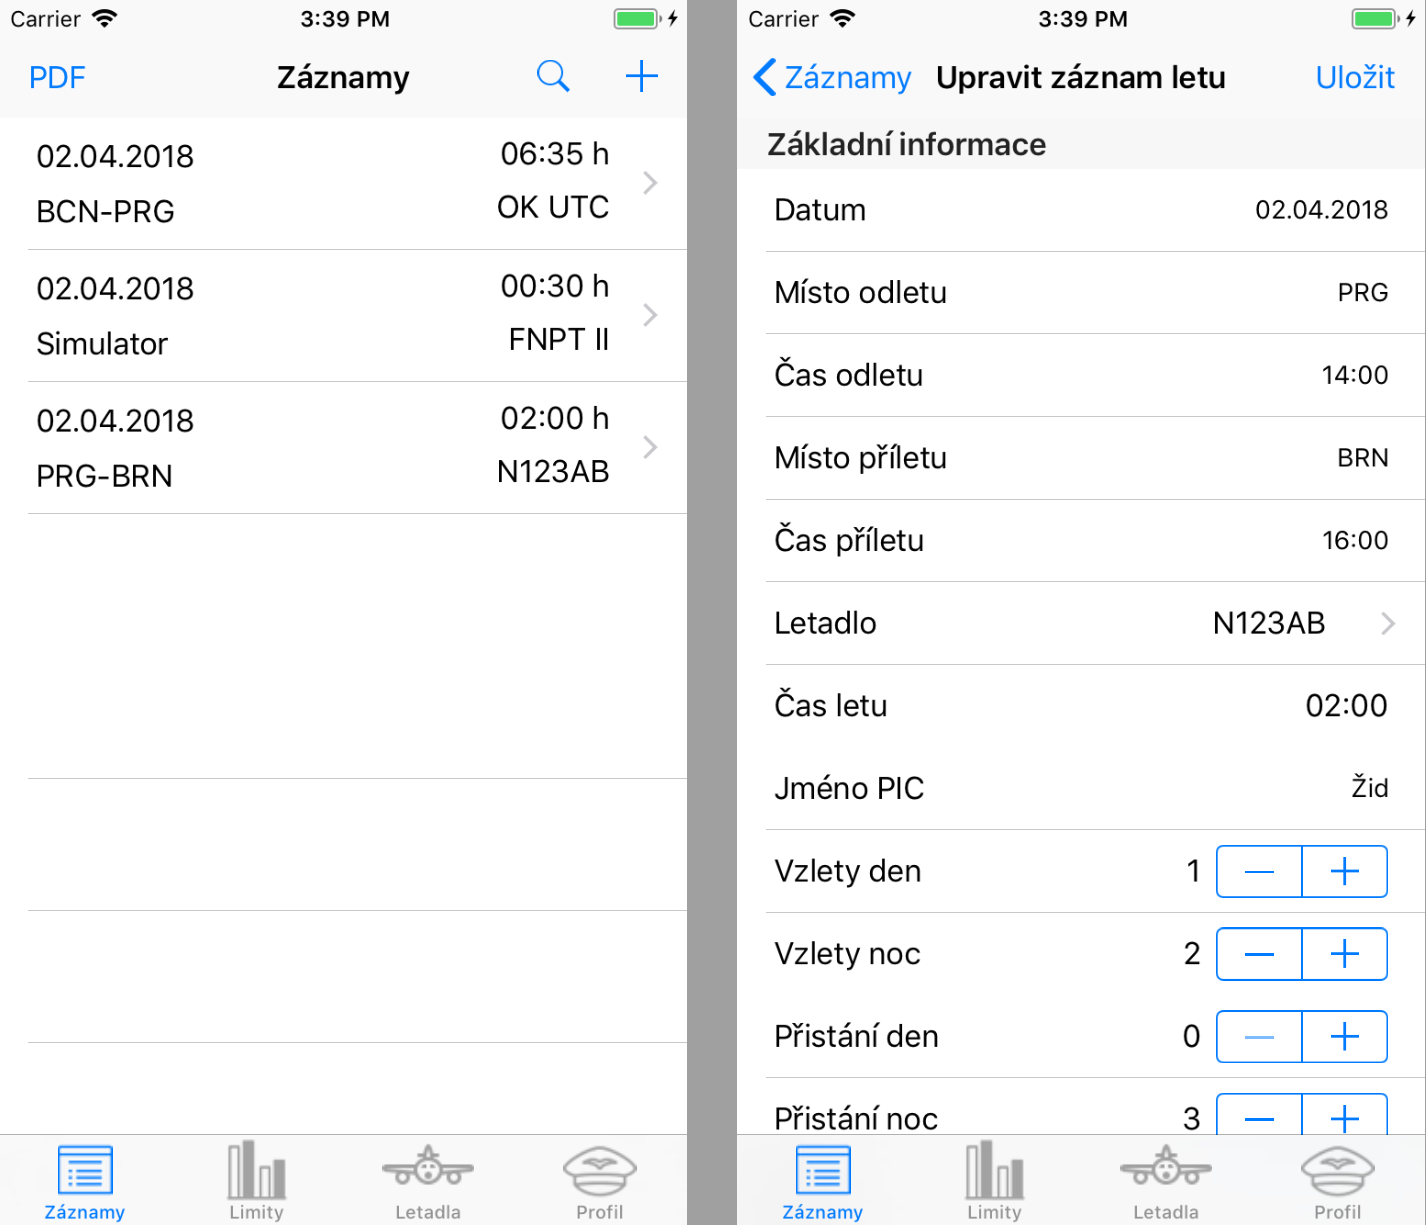
\includegraphics[width=0.99\textwidth]{./pictures/UISplitView/iphone}
 \caption[UISplitViewController na zařízení iPhone 6]{UISplitViewController na zařízení iPhone 6}\label{fig:split1}
\end{figure}

\begin{figure}[]\centering
 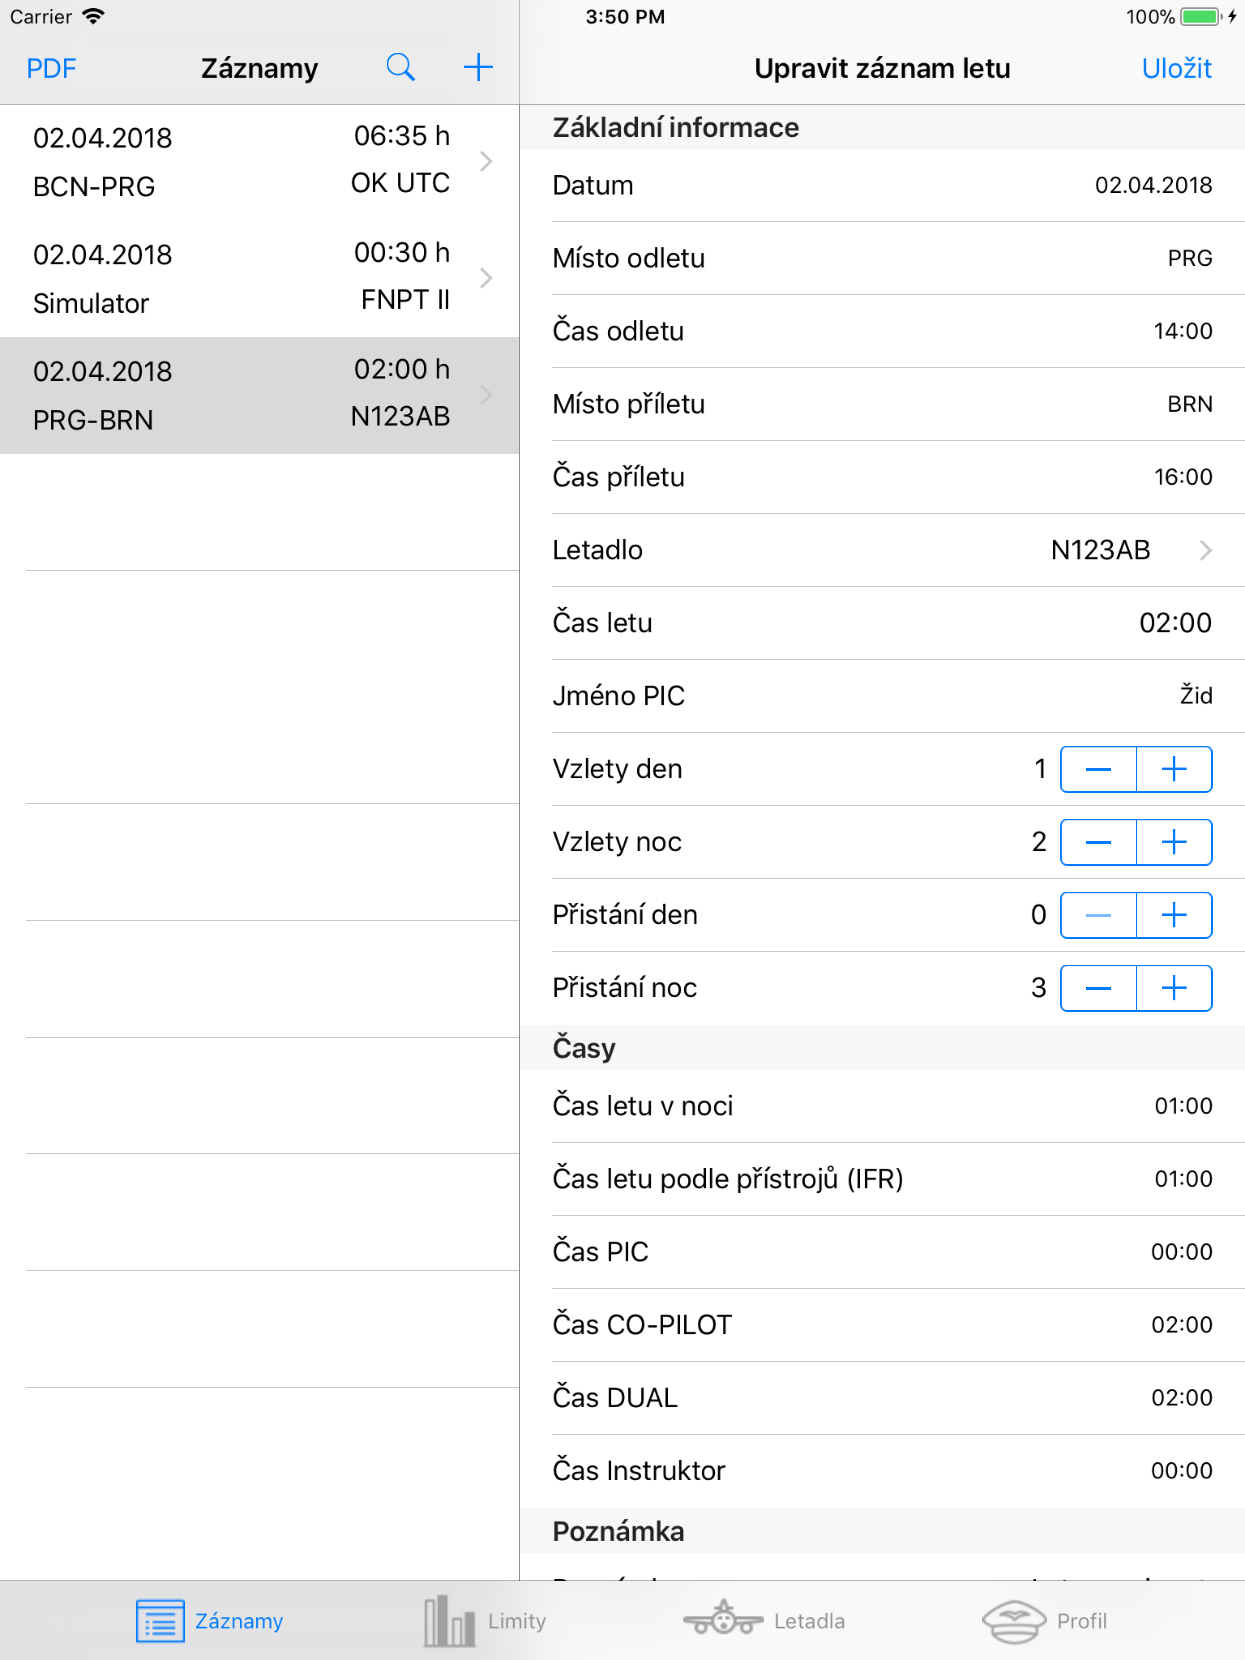
\includegraphics[width=0.99\textwidth]{./pictures/UISplitView/ipad}
 \caption[UISplitViewController na zařízení iPad Air 2]{UISplitViewController na zařízení iPad Air 2}\label{fig:split2}
\end{figure}

\section{Překlady}
U překladů iOS aplikací je nutné uvést dva pojmy -- internacionalizaci a lokalizaci. Internacionalizace je proces zmezinárodnění aplikace, tedy upravení metadat na App Storu, zacílení marketingu, přizpůsobení kulturám daných zemí a lokalizace aplikace. Lokalizace je tedy součást internacionalizace, obsahuje části jako překlady, upravení formátu dat nebo změnění jednotek cen, váhy apod. \cite{internationalization}

Celá aplikace je nyní vytvořena v češtině, ale byla vyvíjená tak, aby ji bylo možné přeložit (lokalizovat) do libovolného jazyka.

Soubory připravené pro překlad aplikace jsou dvojího typy -- překlady storyboardů a tzv. $Localizable.string$. Oba typy jsou závislé na tom, jaké jazyky jsou nastaveny v Xcode projektu.

Soubory pro překlad storyboardů vytváří samotné Xcode. Každý UI prvek je identifikován vygenerovaným ID, které je spojeno s textem, který daný prvek obsahuje. Ukázka storyboardu připraveného pro překlad je zobrazena na příkladu \ref{lst:storyboardLoc}. Tento příklad zobrazuje českou verzi textů storyboardu. Při překladech by došlo k vygenerování např. anglické verze, kde by všechny prvky měli stejné ID jako u české verze a podle nich by došlo k přeložení příslušných textů. Tento způsob překladů byl použit u neměnících se textů prvků ze storyboardů.

Druhý způsob byl použit u textů, které se mohou měnit po spuštění aplikace nebo nejsou definované ve storyboardech. Tento způsob používá soubory $Localizable.string$, kde každý překládaný jazyk má svůj vlastní soubor. Každý z těchto souborů obsahuje dvojice klíč-hodnota, kde klíč představuje ID a hodnota text. Získání hodnoty je možné pomocí $NSLocalizedString$, který vrací přiřazený lokalizovaný text podle zadaného klíče. Ukázka použití $Localizable.string$ je zobrazena na příkladu \ref{lst:locString}.

\begin{figure}
\begin{minipage}{\linewidth}
\begin{lstlisting}[caption={Ukázka přípravy storyboardu pro překlad},label={lst:storyboardLoc}]
/* Class = "UILabel"; text = "Datum";
 ObjectID = "bPZ-q2-xLN";
 */
"bPZ-q2-xLN.text" = "Datum";
...
\end{lstlisting}
\end{minipage}
\end{figure}

\begin{figure}
\begin{minipage}{\linewidth}
\begin{lstlisting}[caption={Ukázka použití $Localizable.string$},label={lst:locString}]
// Localizable.string
"Plane" = "Letadlo";

// get localized Plane
let label = NSLocalizedString("Plane", comment: "")
\end{lstlisting}
\end{minipage}
\end{figure}

\section{Generování PDF}
Tato sekce se zabývá způsobem generování reportu do formátu PDF. Jedná se o funkcionalitu, kde je možné z vybraných záznamů letů a záznamů ze simulátoru vygenerovat report do formátu PDF ve stylu zápisníku letů Jeppesen (\url{http://www.transair.co.uk/sp+Jeppesen-European-Pilot-Logbook-EU-FCL-050+5946}).

Při generování PDF reportu je vytvořena nejprve tabulka ve formátu HTML, ta je vyplněna daty a až z tohoto HTML souboru je generován PDF report. HTML tabulka je v kódu postupně skládána z několika HTML souborů:
\begin{itemize}
\item layout.html -- obsahuje základní definici HTML stránky společně s CSS stylováním,
\item table.html -- obsahuje samotnou definici tabulky tedy rozložení sloupců  a hlavičkové buňky,
\item všechny ostatní soubory s přívlastkem $row$ -- jsou řádky tabulky, které jsou v postupně generovány, vyplňovány a nakonec vloženy do tabulky.
\end{itemize}
Postupné skládání tabulky je zajištěno pomocí značek (začínající znakem \#) v HTML souborech. Tyto soubory jsou načteny ve formě $Stringu$ a následně, pomocí funkce $replacingOccurrences(of:with:)$, jsou jednotlivé značky nahrazovány reálným obsahem. Ukázku tohoto postupného skládání HTML souboru zobrazuje příklad \ref{lst:PDFGen}. Pomocí tohoto postupu jsou tedy vyplňována uživatelova data, počítány statistiky a připraveny překlady.

Pro následné vytvoření PDF reportu byly použity dvě třídy z UIKit -- $UIMarkupTextPrintFormatter$ a $UIPrintPageRenderer$. První z nich se starala o připravení tisknutelného obsahu z HTML souboru. A od druhé dědila vlastní třída $CustomPrintPageRenderer$, která zajišťovala vykreslení (i několika stránek) PDF souboru.  

\begin{figure}
\begin{minipage}{\linewidth}
\begin{lstlisting}[caption={Ukázka postupného skládání HTML souboru},label={lst:PDFGen}]
// layout.html
<!doctype html>
<html>
...
   <body>
      #TABLE
   </body>
</html>

// ViewModel
private struct Marks {
   static let table = "#TABLE"
}

func generateHTMLString() -> String? {
   ...
   // get path to layout.html
   let pathToLayout = Bundle.main
      .path(forResource: HTMLFiles.layout, ofType: html)
   // convert HTML file to String
   var layout = try String(contentsOfFile: pathToLayout!)
   // replace #TABLE with actual tables
   layout = layout.replacingOccurrences(of: Marks.table, 
               with: try generateTables())
   ...
}

private func generateTables() throws -> String {
   ...
}
\end{lstlisting}
\end{minipage}
\end{figure}

\section{Dokumentace}
Společně s implementací aplikace byla vytvořena i její dokumentace. Při psaní kódu byly dodržovány Apple \uv{Design Guidelines} a byla tedy snaha o psaní tzv. self explanatory kódu. Kód byl doplňován komentáři -- proč daná část kódu dělá to, co dělá. 

Samotná dokumentace byla poté zaměřena hlavně na veřejnou část tříd a na složitější metody. Pro tvorbu dokumentace bylo použito oficiální \\Apple značení (markup). A po dokončení aplikace byla dokumentace vygenerována pomocí programu \uv{Jazzy} (\url{https://github.com/realm/jazzy}) do formátu HTML.

Vygenerovaná dokumentace k je nalezení v příloze této diplomové práce. 

\section{Použité nástroje při vývoji}
\subsection{Xcode}
Xcode 9 byly použity pro vývoj, testování a simulování vytvářené aplikace. 

Xcode je software od Applu pro operační systém macOS a používá se pro vývoj aplikací na Mac, iPhone, iPad, Apple Watch a Apple TV. Xcode obsahují zabudované nástroje pro psání kódu, kompilaci, testování, vytváření uživatelského rozhraní, spouštění vytvářené aplikace na simulátorech a další. \cite{Xcode}

\subsection{Git}
Software Git byl používán pro zálohování, verzování a sdílení zdrojových kódů aplikace. 

Git je open source software, který je zdarma a používá se pro verzování projektů. \cite{git}

Repositář aplikace vyvíjené v rámci této diplomové práce byl uložen na GitHub (\url{https://github.com/MartinZid/FlightRecords}). Do tohoto repositáře byl přidán vedoucí této práce jako tzv. collaborator. Díky tomu byl stále informován o změnách a mohlo docházet k revizi zdrojových kódů.

\subsection{Carthage}
Carthage je software, který se používá pro správu frameworků. Carthage tyto frameworky stáhne a připraví pro vložení do projektu, dále je také možné pomocí Carthage frameworky aktualizovat na novější verze. \cite{carthage}

Seznam použitých frameworků je uložen v souboru Cartfile, kde je možné i uvést požadovanou verzi frameworku. Pro stažení a připravení frameworků se používá příkaz $carthage$ $update$. Poté, co jsou frameworky připraveny, je nutné je vložit do Xcode projektu. \cite{carthage}

Pomocí Carthage byly spravovány frameworky:
\begin{itemize}
\item ReactiveCocoa, který obsahuje i ReactiveSwift a Result. Tento framework je licencován pod licencí MIT a je k nalezení na adrese:\\ \url{https://github.com/ReactiveCocoa/ReactiveCocoa/}.
\item Realm k nalezení na adrese: \url{https://realm.io/docs/swift/latest/}.
\item Toast-Swift, který je také licencován pod MIT a je k nalezení na adrese: \url{https://github.com/scalessec/Toast-Swift}.
\end{itemize}

\subsection{Realm Studio}
Realm Studio je vývojářský nástroj vytvořený pro správu Realm databází. V Realm Studiu je možné se připojit na lokální Realm, spravovat jakoukoliv instanci objektového serveru Realm nebo se připojit na Realm Cloud. Realm Studio je dostupné pro Mac, Linux i Windows. \cite{realmStudio}

Realm Studio umožňuje upravovat záznamy v databázi, vytvářet a spravovat uživatele, dotazovat se nad záznamy, zobrazovat logy a další. \cite{realmStudio}

Při vývoje aplikace bylo Realm Studio použito pro testování, ladění a správu databáze.

\chapter{Testování}
Tato kapitola se zabývá jednotkovými (unit) testy, které byly tvořeny v průběhu tvorby aplikace, dále také heuristickou analýzou, uživatelskými testy a nakonec také úpravami, které byly po dokončení testování provedeny.

\section{Unit testy}
Unit testy, neboli jednotkové testy, jsou zaměřeny na části (jednotky) kódu. Těmito jednotkami jsou v objektově orientovaném programování např. funkce nebo třídy. \cite{unitTesting}

Pro tvorbu unit testů ve vytvářené aplikaci byl použit framework XCTest, který je vytvořen společností Apple a má předpřipravené rozhraní v Xcode. \cite{appleTesting}

Všechny testující třídy jsou podtřídou $XCTestCase$. $XCTestCase$ je základní třídou všech testovacích případů. Tato třída obsahuje metody $setUp$ -- umožňující nastavit výchozí stav před testováním, $tearDown$ -- umožňující \uv{uklizení} po skončení testů. Dále tato třída také obsahuje funkce pro vyhodnocení jednotlivých testů. Mezi tyto funkce patří: $XCTAssertEqual$ potvrzující, že dvě vstupní hodnoty jsou stejné; $expectation$ je spojováno s $waitForExpectations$, které čeká danou dobu na to, zda je $expectation$ vyplněno ($fulfill$); a další. Funkce definující testy jsou, v testovací třídě, označeny klíčovým slovem $test$, které je na začatku jejich názvu. Takto definované funkce jsou automaticky spouštěny a vyhodnocovány. Díky klíčovému slovu $test$ je možné definovat i pomocné funkce. \cite{XCTestCase}

Pro třídy, které testují funkce pracující s databází Realm, byla vytvořena testovací třída $XCTestCase$. Tato třída se starala o konfiguraci instance Realmu, která byla pouze v paměti a tudíž testy probíhali stále stejně a neovlivňovali klasickou Realm databázi.

Příklad \ref{lst:unitTests} zobrazuje obě dříve zmíněné funkce -- $setUp$ vytvářející $ViewModel$, který bude podléhat testům a $tearDown$, která $ViewModel$ znovu dealokuje. Následně jsou na ukázce zobrazeny dva testy. 

První z nich testuje, zda jsou $Observeři$ na $Signalu$ informování o tom, že data z Realmu jsou připravena. U tohoto testu je použita dvojice $expectation$ a $waitForExpectations$. $Expectation$ je vyplněno právě, pokud je na $Signal$ odeslána hodnota indikující dokončení přípravy Realmu. 

Druhý test také pracuje s instancí Realmu. Zde je ovšem klasická instance nahrazena instancí s konfigurací $in$ $memory$, protože dochází k zápisu do Realmu. Testováno je zde pomocí $XCTAssertEqual$, zda funkce $numberOfRecordsInSection$ správně reflektuje počet záznamů v databázi Realmu.

Výsledek testů je zobrazen na obrázku \ref{fig:testsResult}.

\begin{figure}[]\centering
 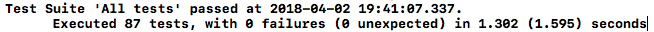
\includegraphics[width=0.99\textwidth]{./pictures/tests}
 \caption[Výsledky testů]{Výsledky testů}\label{fig:testsResult}
\end{figure}

\begin{figure}
\begin{minipage}{\linewidth}
\begin{lstlisting}[caption={Ukázka unit testů},label={lst:unitTests}]
@testable import FlightRecords
...
class RecordsViewModelTests: TestCaseBase {
   var viewModelUnderTest: RecordsViewModel!
    
   override func setUp() {
      super.setUp()
      viewModelUnderTest = RecordsViewModel()
   }
    
   override func tearDown() {
      viewModelUnderTest = nil
      super.tearDown()
   }

   func testRealmSetUpInformingOberversOnComplete() {
      let promise = expectation(description: 
         "observers recieved notification") 
      viewModelUnderTest.collectionChangedSignal
         .observeValues { changes in
         promise.fulfill()
      } 
      waitForExpectations(timeout: 5, handler: nil)
   }

   func testNumberOfRecords() {
      viewModelUnderTest.realm = setUpRealm()
      try! viewModelUnderTest.realm.write {
         viewModelUnderTest.realm.add(Record())
         viewModelUnderTest.realm.add(Record())
      }
      viewModelUnderTest.realmInitCompleted() 
      let numberOfRecords = 
         viewModelUnderTest.numberOfRecordsInSection()  
      XCTAssertEqual(numberOfRecords, 2, 
         "Number of records is wrong.")
   }
   ...
}
\end{lstlisting}
\end{minipage}
\end{figure}
	
\section{Heuristická analýza}
Heuristická analýza byla provedena znovu poté, co byla aplikace implementována do stavu tzv. beta verze aplikace. I tato heuristická analýze byla prováděna podle pravidel Jakoba Nielsena a nyní již bylo zohledněno všech deset pravidel. Všechny nalezené chyby, stejně jako u předchozí heuristické analýzy, byly ohodnoceny na stupnici 1--5, kde číslo 1 identifikuje pouze drobný problém a číslo 5 velice závažný problém. U všech nalezených problémů je také uvedeno řešení, pomocí kterého byly chyby opraveny. Nakonec tabulka \ref{tab:heu_eval_2} zobrazuje u každého pravidla, zda bylo porušeno a jaká byla maximální závažnost porušení tohoto pravidla.

\begin{enumerate}

\item Viditelnost stavu systému -- 
\begin{itemize}
	\item Uživatel není explicitně informován o tom, že jsou záznamy filtrovány.
 	\begin{itemize}
 		\item Závažnost problému -- 4.
 		\item Řešení -- přidání informující záložky, která umožňuje i zrušení filtrování.
 	\end{itemize}
 	\item Pokud neexistují žádné záznamy letů (ze simulátoru) nebo letadel, uživateli je zobrazena pouze prázdná tabulka.
 	\begin{itemize}
 		\item Závažnost problému -- 3.
 		\item Řešení -- přidání zprávy, která bude informovat uživatele, že žádné záznamy (letů, ze simulátoru a letadel) neexistují.
 	\end{itemize}
 	\item Pokud parametrům filtrování neodpovídají žádné záznamy, je uživateli zobrazena prázdná tabulka.
 	\begin{itemize}
 		\item Závažnost problému -- 2.
 		\item Řešení -- přidání zprávy informující uživatele o tom, že parametrům filtrování neodpovídají žádné záznamy. 	
 	\end{itemize}
 	\item Uživatel není informován o úspěšném přidání záznamu/letadla.
 	\begin{itemize}
 		\item Závažnost -- 2.
 		\item Řešení -- po přidání záznamu/letadla bude uživateli zobrazena hláška o úspěšném přidání.
 	\end{itemize}
 	\item Zobrazení náhledu reportu a generování PDF může trvat delší dobu.
 	\begin{itemize}
 		\item Závažnost -- 3.
 		\item Řešení -- uživatel je informován o tom, že aplikace pracuje pomocí tzv. spinner. 
 	\end{itemize}
\end{itemize}
 
\item Spojení systému a reálného světa -- 
\begin{itemize}
 	\item Název \uv{Limity} je příliš obecný.
 	\begin{itemize}
 		\item Závažnost -- 1.
 		\item Řešení -- přejmenování \uv{Limity} na \uv{Limity nalétaných hodin}.
 	\end{itemize}
 	\item Popis \uv{Typ} při přidávání/upravě záznamu ze simulátoru nemusí jasně specifikovat, že se má jednat o typ simulátoru (zařízení).
 	\begin{itemize}
 		\item Závažnost -- 2.
 		\item Řešení -- přejmenování popisu \uv{Typ} na \uv{Typ zařízení}.
 	\end{itemize}
\end{itemize}
 
\item Uživatelská kontrola a volnost -- 
\begin{itemize}
	\item Smazání záznamu nebo letadla je definitivní.
	\begin{itemize}
		\item Závažnost problému -- 4.
		\item Řešení -- podpora funkce vrácení zpět (tzv. undo).
	\end{itemize}
\end{itemize}
 
\item Konzistence a standardizace -- 
\begin{itemize}
 	\item Nebyl nalezen problém.
\end{itemize}
 
\item Předcházení chyb -- 
\begin{itemize}
 	\item Uživatel může omylem smazat záznam nebo letadlo.
 	\begin{itemize}
 		\item Závažnost -- 4.
 		\item Řešení -- zobrazení dialogového okna s potvrzením uživatelovi akce.
 	\end{itemize}
\end{itemize}
 
\item Rozpoznání místo vzpomínání -- 
\begin{itemize}
 	\item Nebyl nalezen problém.
\end{itemize}
 
\item Flexibilita a efektivita použití -- 
\begin{itemize}
 	\item Nebyl nalezen problém.
\end{itemize}
 
\item Estetika a minimalismus --
\begin{itemize}
\item Při nastavování filtrování se uživateli zbytečně zobrazují položky \uv{Typ letadla} a \uv{Letadlo} pokud uživatel vyhledává pouze záznamy ze simulátoru.
\begin{itemize}
	\item Závažnost -- 3.
	\item Řešení -- skrývání zbytečných položek při specifickém nastavení filtrování.
\end{itemize}
\end{itemize}  
  
\item Pomoci uživatelům rozpoznat, pochopit a vzpamatovat se z~chyb -- 
\begin{itemize}
\item Uživatel není informován o tom, že se nepodařilo přihlásit pomocí jeho iCloud účtu.
\begin{itemize}
	\item Závažnost -- 4.
	\item Řešení -- zobrazení chybové hlášky informující uživatele o chybě a poskytující informace dostatečné  k tomu, aby se uživatel z chyby vzpamatoval.
\end{itemize}
\end{itemize}

\item Nápověda a dokumentace -- 
\begin{itemize}
 	\item Nebyl nalezen problém při zohlednění cílové skupiny uživatelů.
\end{itemize}
\end{enumerate}

\begin{table}[h] \centering
\begin{tabular}{ l | c | c |}
 Bod & Rozpor & Max. závažnost\\
\hline
 1 & \OK & 4 \\
 2 & \OK & 2 \\
 3 & \OK & 4 \\
 4 & \NOK & - \\
 5 & \OK & 4 \\
 6 & \NOK & - \\
 7 & \NOK & - \\
 8 & \OK & 3 \\
 9 & \OK & 4 \\
 10 & \NOK & - \\
\end{tabular}
\caption[Závažnosti prorušení pravidel]{Závažnosti prorušení pravidel}\label{tab:heu_eval_2}
\end{table}

\section{Uživatelské testování}
Uživatelské testování proběhlo ihned po heuristické analýze. Testováni byli celkem čtyři uživatelé, kteří byly rozděleni na dvě skupiny -- ti, co mají znalosti v oboru letectví a ostatní. U všech uživatelů bylo podmínkou používání operačního systému iOS po dobu alespoň dvou let. Všichni uživatelé dostaly stejné otázky před začátkem testování, stejné scénáře a stejný závěrečný dotazník. Skupině uživatelů, která neměla znalosti v leteckém oboru, byly nejprve vysvětleny základní informace nutné k plynulému absolvování testů.

Všechny testy byly nahrávány z důvodu možné zpětné analýzy nedostatků aplikace. Všechny nahrávky testů společně s vyplněnými dotazníky jsou k nalezení v příloze této diplomové práce.

Před samotným testováním byli uživatelé seznámeni s testovacími scénáři (z důvodu vysvětlení nejasností) a odpovídali na několik otázek. Dále byli vyzvání ke komentování svých myšlenek v průběhu testování a také byli ujištěni o tom, že pokud cokoliv nepůjde, tak to není jejich chyba, ale chyba aplikace.

\subsection{Základní otázky na testované uživatele}
\begin{enumerate}
\item Jak dlouho používáte iOS?
\item Jaké zařízeni od Applu máte?
\item Jste právě teď přihlášeni do účtu iCloud?
\item Je toto Vaše první uživatelské testování?
\end{enumerate}

\subsection{Scénáře}
Testovací scénáře byly lehce upraveny a rozšířeny oproti scénářům použitým na otestování návrhu uživatelského rozhraní.

\begin{enumerate}
\item Právě jste dokončil(a) svůj první let z Brna do Prahy. Z Brna jste odlétal(a) v 7:00 a do Prahy jste přiletěl(a) v 8:45, neměl(a) jste žádné mezipřistání. Celou doby jste zastával(a) funkci vedoucího pilota a letěl(a) jste letadlem Boeing. Zaznamenejte svůj let.
\item Zjistil(a) jste, že jste u minulého záznamu chybně zaznamenal(a) čas. Upravte tedy čas příletu do Prahy na 7:45.
\item Chcete si přidat další záznam, tentokrát z výcvikového zařízení. Zadejte dnešní datum, čas na zařízení dvě hodiny.
\item Zadejte do aplikace další dva záznamy. Vyplňované hodnoty jsou na Vás, pouze datum specifikujte na minulý týden.
\item Pokuste se vyfiltrovat záznamy tak, aby se Vám zobrazovaly pouze záznamy letů z minulého týdne.
\item Jeden ze záznamů z minulého kroku smažte.
\item Vyplňte si osobní informace (nemusí být pravdivé).
\item U letadla Boeing z prvního kroku chcete změnit model. Proveďte tuto úpravu.
\item Za poslední tři týdny jste absolvoval(a) mnoho letů, zkontrolujte, zda jste nepřekročil(a) jeden z limitů.
\item Zjistěte kolik jste celkově nalétal(a) s Vaším letadlem Boeing.
\item Dnes Vám vydali zdravotní certifikát třídy jedna (Class 1). Vložte ho do aplikace.
\item Vytvořte report ze všech záznamů letů i záznamů z výcvikového zařízení za posledních čtrnáct dní a odešlete si tento report na email.
\end{enumerate}

\subsection{Závěrečný dotazník}
Jako závěrečný dotazník byl zvolen SUS -- \uv{System Usability Scale}, který se používá pro měření uživatelského vnímání použitelnosti produktu. SUS obsahuje deset otázek:
\begin{enumerate}
 \item \uv{rád bych používal systém opakovaně,
 \item systém je zbytečně složitý,
 \item systém se snadno používá,
 \item potřeboval bych pomoc od člověka z~technické podpory, abych mohl systém používat,
 \item různé funkce systému jsou dobře zakomponované,
 \item systém je nekonzistentní,
 \item myslím si, že se většina lidí se se systémem rychle naučí,
 \item systém se těžko ovládá,
 \item jsem si jistý(á) při používání tohoto systému,
 \item potřebuji se naučit mnoho věcí, než začnu používat tento systém} (překlad vlastní).
\end{enumerate}
Ke každé otázce je odpověď s~výběrem z~pěti možností. Odpovědi jsou ohodnoceny 1--5, kde 1 představuje silný nesouhlas a 5 silný souhlas. \cite{sus}

\subsection{Výsledky testů}
Tabulka \ref{tab:ut_eval} zobrazuje hodnocení splnění scénářů u jednotlivých uživatelů. Hodnocení bylo znovu v rozsahu 1 až 5, kde 1 představuje bezproblémové splnění a 5 nedokončení scénáře.  Z tabulky je možné vidět, že všichni uživatelé nějakým způsobem splnily všechny zadané scénáře (nejhorší hodnocení je 4 a to se objevuje pouze jednou). Je také možné si všimnout, že pokud některé scénáře obsahovaly podobné kroky, jako scénáře již absolvované (např. filtrování nebo vkládání záznamu), uživatelé se s aplikací již seznámili a naučili a s dalšími obdobnými úlohami již neměli problém.

\begin{table}\centering
 \begin{tabular}{ c | c | c | c | c |}
 	 & Uživatel 1 & Uživatel 2 & Uživatel 3 & Uživatel 4 \\
 	\hline
 	Úloha 1  & 2 & 2 & 1 & 2 \\
 	Úloha 2  & 1 & 1 & 1 & 1 \\
 	Úloha 3  & 1 & 1 & 1 & 1 \\
 	Úloha 4  & 1 & 2 & 3 & 1 \\
 	Úloha 5  & 1 & 2 & 1 & 1 \\
 	Úloha 6  & 1 & 1 & 3 & 1 \\
 	Úloha 7  & 1 & 1 & 1 & 1 \\
 	Úloha 8  & 1 & 4 & 1 & 1 \\
 	Úloha 9  & 1 & 1 & 1 & 1 \\
 	Úloha 10 & 3 & 2 & 3 & 3 \\
 	Úloha 11 & 1 & 1 & 1 & 1 \\
 	Úloha 12 & 1 & 1 & 2 & 3 \\
 \end{tabular}
 \caption[Hodnocení splnění jednotlivých scénářů]{Hodnocení splnění jednotlivých scénářů}\label{tab:ut_eval}
\end{table}

Při testování nebyly objeveny žádné kritické problémy, však díky pozorování a nahrávání uživatelů bylo objeveno několik nedostatků, které byly následně opraveny. Zde je jejich seznam.

\begin{itemize}
\item Při přidávání nebo úpravě záznamu letů již nemizí určité řádky tabulky (opraveno již po prvním testování).
\item Certifikát, který není pojmenovaný se nyní v tabulce označuje jako \uv{Nepojmenovaný}. Dříve nebyl označený nijak.
\item U certifikátů s dlouhým názvem již není zobrazen celý název, ale pouze určitá část.
\item U záložek, které obsahují $UISplitViewController$ již funguje vrácení se na hlavní stránku záložky, při dvojím poklepání na danou záložku.
\item Zaměření textového pole je nyní možné při kliknutí kamkoliv na řádek s tímto textovým polem.
\item Řádky statických tabulek jsou nyní zvýrazňovány pouze pokud obsahují nějakou akci.
\item Akce \uv{Zrušit filtrování} je potvrzována dialogovým oknem.
\item U filtrování je nyní možné zrušit nastavené letadlo.
\item Při odesílaní reportu na email je nyní uživatel informován pokud nemá nastaveny emailový klient.
\end{itemize}

\chapter{Zhodnocení}
Tato kapitola se zabývá zhodnocením postupů FRP -- jejich výhodami a nevýhodami, a dále také zhodnocením časové a implementační náročnosti při vývoji aplikace za pomocí FRP a architektury MVVM v porovnání se standardním přístupem architektury MCV.

\section{Zhodnocení postupů FRP v aplikaci}
Postupy funkcionálně reaktivní programování velice dobře  vyhovují požadavkům, které jsou kladeny na mobilní aplikace --  prezentování uživatelského rozhraní a neustálé reagování na změny, které mohou přijít jak od uživatele, tak i např. ze serveru. Díky FRP je možné všechny tyto změny pozorovat ve formě nezávislých datových toků a podle nich následně upravovat uživatelské rozhraní a to bez nutnosti složitého uchovávání stavů aplikace.

ReactiveCocoa se prokázala jako velice kvalitní framework pro tvorbu reaktivní iOS aplikace. Nejen, že tento framework poskytuje řadu základní reaktivní prvků, on také přidává komponentám uživatelského rozhraní reaktivní rozšíření, čímž umožňuje vytvořit plně reaktivní aplikaci.

Za zmínku zde stojí i Realm, který se dal velice jednoduše zkombinovat s frameworkem Reactive Cocoa. Kde pozorované změny např. na Realm kolekcích byly transformovány na $Signal$, na který následně reagovalo uživatelské rozhraní. Tímto postupem bylo dosaženo např. toho, že aplikace automaticky reagovala na každou změnu v Realmu, bez nutnosti jakékoliv uživatelovi iniciativy o znovu načtení dat.

Postupy FRP tedy přináší mnoho výhod, které ulehčují tvorbu mobilních aplikací. Je zde však nutné zmínit i pár nevýhod tohoto přístupu. Prvním drobným nedostatkem je to, že postupy FRP není možné zavést v rámci standardních Apple knihoven a je nutné použít neoficiální frameworky (tedy další knihovny/frameworky navíc). Další nevýhodou je to, že je nutné se seznámit se zcela novým programovacím stylem a tedy, i přizpůsobit to, jakým způsobem přemýšlíme nad problémy. Tato nevýhoda se projevuje hlavně na začátku, při přechodu od klasického tzv. imperativního stylu programovaní k FRP, a je později zcela zastíněna tím, že dochází k tvorbě nezávislých komponent, které jsou schopné reagovat na danou změnu pomocí velice přehledného a elegantního kódu.

\section{Zhodnocení časové a implementační náročnosti MVVM a FRP oproti MVC}
Stejně jako postupy FRP, tak i architektura MVVM přinesla mnoho prospěšných aspektů. Tato architektura přidává novou vrstvu, která je zcela nezávislá na $View$. Tento fakt, může evokovat zbytečné zkomplikování struktury aplikace, však v tomto případě tomu tak jistě není. Nová vrstva $ViewModel$ je nejčastěji použita jedna ku jedné se třídami $ViewControllerů$ a jedná se hlavně o oddělení logiky -- té, co se zabývá $View$ a ostatní. Díky tomuto rozdělení obsahují $ViewControllery$ méně kódu a jsou daleko přehlednější.

Tedy, i když je ke každému $ViewControlleru$ vytvářen pokaždé soubor $ViewModelu$ navíc, celkově je aplikace lépe upravitelná, rozšířitelná a obsahuje komponenty, které splňují tzv. \uv{single responsibility principle} a jsou často znovupoužitelné.

Architektura MVVM skvěle funguje ve spojení s funkcionálně reaktivním programováním, které se dokáže postarat o jednoduché spojení vrstev $View$ a $ViewModelu$.

Jak je již zmíněno dříve, FRP může být časově náročnější hlavně zpočátku při přechodu od klasického imperativního stylu. Toto je později zastíněno všemi výhodami, které FRP přináší (mezi něž patří i zjednodušení a urychlení implementace).

Klasické postupy společně s architekturou MVC se tedy hodí pouze pro velice malé a jednoduché aplikace. Jakmile začne být aplikace lehce komplexnější, architektura MVVM ve spojení s FRP se, jak z pohledu časové tak i implementační náročností, vyplatí.

\begin{conclusion}

	%sem napište závěr Vaší práce
\end{conclusion}

\bibliographystyle{csn690}
\bibliography{mybibliographyfile}

\appendix

\chapter{Seznam použitých zkratek}
% \printglossaries
\begin{description}
	\item[FRP] Funkcionálně reaktivní programování
	\item[MVC] Model View Controller
	\item[MVVM] Model View ViewModel
	\item[VIPER] View Interactor Presenter Entity Router
	\item[PC] Personal Computer
	\item[EASA] European Aviation Safety Agency
	\item[PIC] Pilot-in-command
	\item[SE] Single engine
	\item[ME] Multi engine
	\item[SPIC] Student PIC
	\item[PICUS] PIC under supervision
	\item[FSTD] flight simulation training devices
	\item[FI] Flight instructor
	\item[FE] Flight examiner
	\item[LAPL] Light Aircraft Pilot Licence
	\item[SPL] Sailplane Pilot Licence
	\item[BPL] Balloon Pilot Licence
	\item[PPL] Private Pilot Licence
	\item[SUS] System Usability Scale
\end{description}


% % % % % % % % % % % % % % % % % % % % % % % % % % % % 
% % Tuto kapitolu z výsledné práce ODSTRAŇTE.
% % % % % % % % % % % % % % % % % % % % % % % % % % % % 
% 
% \chapter{Návod k~použití této šablony}
% 
% Tento dokument slouží jako základ pro napsání závěrečné práce na Fakultě informačních technologií ČVUT v~Praze.
% 
% \section{Výběr základu}
% 
% Vyberte si šablonu podle druhu práce (bakalářská, diplomová), jazyka (čeština, angličtina) a kódování (ASCII, \mbox{UTF-8}, \mbox{ISO-8859-2} neboli latin2 a nebo \mbox{Windows-1250}). 
% 
% V~české variantě naleznete šablony v~souborech pojmenovaných ve formátu práce\_kódování.tex. Typ může být:
% \begin{description}
% 	\item[BP] bakalářská práce,
% 	\item[DP] diplomová (magisterská) práce.
% \end{description}
% Kódování, ve kterém chcete psát, může být:
% \begin{description}
% 	\item[UTF-8] kódování Unicode,
% 	\item[ISO-8859-2] latin2,
% 	\item[Windows-1250] znaková sada 1250 Windows.
% \end{description}
% V~případě nejistoty ohledně kódování doporučujeme následující postup:
% \begin{enumerate}
% 	\item Otevřete šablony pro kódování UTF-8 v~editoru prostého textu, který chcete pro psaní práce použít -- pokud můžete texty s~diakritikou normálně přečíst, použijte tuto šablonu.
% 	\item V~opačném případě postupujte dále podle toho, jaký operační systém používáte:
% 	\begin{itemize}
% 		\item v~případě Windows použijte šablonu pro kódování \mbox{Windows-1250},
% 		\item jinak zkuste použít šablonu pro kódování \mbox{ISO-8859-2}.
% 	\end{itemize}
% \end{enumerate}
% 
% 
% V~anglické variantě jsou šablony pojmenované podle typu práce, možnosti jsou:
% \begin{description}
% 	\item[bachelors] bakalářská práce,
% 	\item[masters] diplomová (magisterská) práce.
% \end{description}
% 
% \section{Použití šablony}
% 
% Šablona je určena pro zpracování systémem \LaTeXe{}. Text je možné psát v~textovém editoru jako prostý text, lze však také využít specializovaný editor pro \LaTeX{}, např. Kile.
% 
% Pro získání tisknutelného výstupu z~takto vytvořeného souboru použijte příkaz \verb|pdflatex|, kterému předáte cestu k~souboru jako parametr. Vhodný editor pro \LaTeX{} toto udělá za Vás. \verb|pdfcslatex| ani \verb|cslatex| \emph{nebudou} s~těmito šablonami fungovat.
% 
% Více informací o~použití systému \LaTeX{} najdete např. v~\cite{wikilatex}.
% 
% \subsection{Typografie}
% 
% Při psaní dodržujte typografické konvence zvoleného jazyka. České \uv{uvozovky} zapisujte použitím příkazu \verb|\uv|, kterému v~parametru předáte text, jenž má být v~uvozovkách. Anglické otevírací uvozovky se v~\LaTeX{}u zadávají jako dva zpětné apostrofy, uzavírací uvozovky jako dva apostrofy. Často chybně uváděný symbol "{} (palce) nemá s~uvozovkami nic společného.
% 
% Dále je třeba zabránit zalomení řádky mezi některými slovy, v~češtině např. za jednopísmennými předložkami a spojkami (vyjma \uv{a}). To docílíte vložením pružné nezalomitelné mezery -- znakem \texttt{\textasciitilde}. V~tomto případě to není třeba dělat ručně, lze použít program \verb|vlna|.
% 
%Více o~typografii viz \cite{kobltypo}.
% 
% \subsection{Obrázky}
% 
% Pro umožnění vkládání obrázků je vhodné použít balíček \verb|graphicx|, samotné vložení se provede příkazem \verb|\includegraphics|. Takto je možné vkládat obrázky ve formátu PDF, PNG a JPEG jestliže používáte pdf\LaTeX{} nebo ve formátu EPS jestliže používáte \LaTeX{}. Doporučujeme preferovat vektorové obrázky před rastrovými (vyjma fotografií).
% 
% \subsubsection{Získání vhodného formátu}
% 
% Pro získání vektorových formátů PDF nebo EPS z~jiných lze použít některý z~vektorových grafických editorů. Pro převod rastrového obrázku na vektorový lze použít rasterizaci, kterou mnohé editory zvládají (např. Inkscape). Pro konverze lze použít též nástroje pro dávkové zpracování běžně dodávané s~\LaTeX{}em, např. \verb|epstopdf|.
% 
% \subsubsection{Plovoucí prostředí}
% 
% Příkazem \verb|\includegraphics| lze obrázky vkládat přímo, doporučujeme však použít plovoucí prostředí, konkrétně \verb|figure|. Například obrázek \ref{fig:float} byl vložen tímto způsobem. Vůbec přitom nevadí, když je obrázek umístěn jinde, než bylo původně zamýšleno -- je tomu tak hlavně kvůli dodržení typografických konvencí. Namísto vynucování konkrétní pozice obrázku doporučujeme používat odkazování z~textu (dvojice příkazů \verb|\label| a \verb|\ref|).
% 
% \begin{figure}\centering
% 	
\includegraphics[width=0.5\textwidth, angle=30]{cvut-logo-bw}
% 	\caption[Příklad obrázku]{Ukázkový obrázek v~plovoucím prostředí}\label{fig:float}
% \end{figure}
% 
% \subsubsection{Verze obrázků}
% 
% % Gnuplot BW i barevně
% Může se hodit mít více verzí stejného obrázku, např. pro barevný či černobílý tisk a nebo pro prezentaci. S~pomocí některých nástrojů na generování grafiky je to snadné.
% 
% Máte-li například graf vytvořený v programu Gnuplot, můžete jeho černobílou variantu (viz obr. \ref{fig:gnuplot-bw}) vytvořit parametrem \verb|monochrome dashed| příkazu \verb|set term|. Barevnou variantu (viz obr. \ref{fig:gnuplot-col}) vhodnou na prezentace lze vytvořit parametrem \verb|colour solid|.
% 
% \begin{figure}\centering
% 	\includegraphics{gnuplot-bw}
% 	\caption{Černobílá varianta obrázku generovaného programem Gnuplot}\label{fig:gnuplot-bw}
% \end{figure}
% 
% \begin{figure}\centering
% 	\includegraphics{gnuplot-col}
% 	\caption{Barevná varianta obrázku generovaného programem Gnuplot}\label{fig:gnuplot-col}
% \end{figure}
% 
% 
% \subsection{Tabulky}
% 
% Tabulky lze zadávat různě, např. v~prostředí \verb|tabular|, avšak pro jejich vkládání platí to samé, co pro obrázky -- použijte plovoucí prostředí, v~tomto případě \verb|table|. Například tabulka \ref{tab:matematika} byla vložena tímto způsobem.
% 
% \begin{table}\centering
% 	\caption[Příklad tabulky]{Zadávání matematiky}\label{tab:matematika}
% 	\begin{tabular}{|l|l|c|c|}\hline
% 		Typ		& Prostředí		& \LaTeX{}ovská zkratka	& \TeX{}ovská zkratka	\tabularnewline \hline \hline
% 		Text		& \verb|math|		& \verb|\(...\)|	& \verb|$...$|		\tabularnewline \hline
% 		Displayed	& \verb|displaymath|	& \verb|\[...\]|	& \verb|$$...$$|	\tabularnewline \hline
% 	\end{tabular}
% \end{table}
% 
% % % % % % % % % % % % % % % % % % % % % % % % % % % % 

\chapter{Obsah přiloženého CD}

%upravte podle skutecnosti

\begin{figure}
	\dirtree{%
		.1 readme.txt\DTcomment{stručný popis obsahu CD}.
		.1 exe\DTcomment{adresář se spustitelnou formou implementace}.
		.1 src.
		.2 impl\DTcomment{zdrojové kódy implementace}.
		.2 thesis\DTcomment{zdrojová forma práce ve formátu \LaTeX{}}.
		.1 text\DTcomment{text práce}.
		.2 thesis.pdf\DTcomment{text práce ve formátu PDF}.
		.2 thesis.ps\DTcomment{text práce ve formátu PS}.
	}
\end{figure}

\end{document}
